\\documentclass{article} 
% \\usepackage{iclr2026_conference,times}
\\usepackage{macros}
\\usepackage{hyperref}
\\usepackage{url}
\\usepackage[toc,page,header]{appendix}
\\usepackage{geometry}
\\geometry{margin=1in}

\\usepackage{minitoc}

\\renewcommand \\thepart{}
\\renewcommand \\partname{}

\\title{Spectral State Space Models for Horizontal Connections and Video Modeling}

\\author{}

\\newcommand{\\greg}[1]{{\\color{indigo}[Gregoire]: #1}}
\\newcommand{\\fel}[1]{{\\color{gold}[Fel]: #1}}
\\newcommand{\\agus}[1]{{\\color{green}[Agus]: #1}}
\\newcommand{\\boutin}[1]{{\\color{pink}[Baltringueur]: #1}}


\\begin{document}

\\doparttoc % Tell to minitoc to generate a toc for the parts
\\faketableofcontents % Run a fake tableofcontents command for the partocs

\\maketitle

\\begin{abstract}
...
\\end{abstract}

\\section{Introduction}

\\section{Related Work}

\\section{Background}

\\subsection{Notations}

\\greg{TODO : put all vectors and matrices in bold}

\\paragraph{Linear Algebra.} Let $\\K$ be a field. We identify $\\mathcal{M}_{m,n}(\\K)$ to $\\K^{m \\times n}$, the set of $m \\!\\times\\! n$ matrices with coefficients in $\\K$. We denote vectors with bold lowercase letters $\\bm x \\in \\K^n$ and linear operators with bold uppercase letters $\\bm A \\in \\K^{m \\times n}$. Scalars are denoted with non bold letters. We write $e^A = \\sum_{k=0}^\\infty \\frac{A^k}{k!}$ the matrix exponential, and $\\sigma(A)$ the spectrum of $A$.

\\begin{thomasbox}
MATRIX EXPONENTIAL. The notation $e^A$ is the matrix exponential, defined as the power series $\\sum_{k=0}^\\infty \\frac{A^k}{k!}$. This is the matrix analog of the scalar exponential function.

WHY IT FOLLOWS: For a square matrix $A$, we can formally substitute $A$ into the Taylor series for $e^x$. The series converges for all square matrices $A$. This is fundamental in solving continuous-time linear ODEs: $h'(t) = Ah(t)$ has solution $h(t) = e^{At}h_0$.

INTUITION: The matrix exponential describes continuous-time linear evolution. For a diagonal matrix $\\Lambda = \\mathrm{diag}(\\lambda_1, \\ldots, \\lambda_N)$, we have $e^{\\Lambda t} = \\mathrm{diag}(e^{\\lambda_1 t}, \\ldots, e^{\\lambda_N t})$, so each eigenvalue evolves independently.
\\end{thomasbox}

\\paragraph{Special Matrices.} $I_n$ is the identity matrix of size $n$. $\\mathrm{Circ}(K) \\in \\R^{n \\times n}$ denotes the circulant matrix generated by the vector $K \\in \\R^n$, possibly zero padded. $\\mathrm{diag}(\\Lambda)$ is a diagonal matrix with diagonal $\\Lambda \\in \\R^n$. For ease of notation, we often identify $\\Lambda$ and $\\mathrm{diag}(\\Lambda)$. $\\Lambda_c$ is a block-diagonal matrix with blocks of size $c \\!\\times\\! c$. Any matrix $\\cdot_c$ notation is block diagonal with blocks of size $c \\!\\times\\! c$. $F_n$ is the Fourier matrix of size $n$.

\\begin{thomasbox}
CIRCULANT MATRICES. A circulant matrix $\\mathrm{Circ}(K)$ is generated by a single vector $K = [k_0, k_1, \\ldots, k_{n-1}]$ with rows that are cyclic shifts of $K$. For example, if $n=3$ and $K = [a, b, c]$, then $\\mathrm{Circ}(K) = \\begin{pmatrix} a & c & b \\\\ b & a & c \\\\ c & b & a \\end{pmatrix}$. The key property is that all circulant matrices are diagonalized by the Fourier matrix: $\\mathrm{Circ}(K) = F^{-1} \\mathrm{diag}(\\hat{K}) F$, where $\\hat{K}$ is the DFT of $K$.

WHY IT FOLLOWS: By definition of the Fourier matrix and the circulant structure. The DFT values are $\\hat{k}_j = \\sum_{m=0}^{n-1} k_m e^{-2\\pi i jm/n}$.

INTUITION: Circulant matrices capture periodic boundary conditions (wraparound). They model convolutions via the FFT because convolution in the spatial domain becomes element-wise multiplication in the Fourier domain.
\\end{thomasbox}

\\begin{thomasbox}
BLOCK-DIAGONAL NOTATION. $\\Lambda_c$ denotes a block-diagonal matrix where each diagonal block is a $c \\times c$ matrix. For example, $\\Lambda_2 = \\begin{pmatrix} A_1 & 0 \\\\ 0 & A_2 \\end{pmatrix}$ where each $A_i$ is $2 \\times 2$. This notation is used because operations on block-diagonal matrices can be parallelized across independent blocks.

WHY IT FOLLOWS: By definition of block-diagonal structure.

INTUITION: Block-diagonal matrices represent systems with independent subsystems. If $\\Lambda_c = Q_c \\Lambda Q_c^{-1}$ where $\\Lambda$ is diagonal and $Q_c$ is block-diagonal, we've diagonalized the block structure, reducing $O(N c^3)$ cost to $O(N c^2)$ or better.
\\end{thomasbox}

\\paragraph{State Space Models.} For the SSMs, we write $x, y \\in \\R^{d}$ the input and output, $h \\in \\R^{N}$ the hidden state, $A \\in \\R^{{N}\\times {N}}$ the transition matrix, $B \\in \\R^{N \\times d}$ and $C \\in \\R^{d \\times N}$ the input and output matrices, respectively. $A$, $\\widetilde{A}$ and $\\widehat{A}$ denote equivalent formulations of a continuous-time SSM while $\\overline{A}$ denotes the discretised version of $A$.

\\begin{thomasbox}
SSM NOTATION CONVENTIONS. In this paper, three types of SSM representations are used:
- $A$: continuous-time transition matrix (from $h'(t) = Ah(t) + Bx(t)$)
- $\\widetilde{A}$: diagonalized or spectral form (change of basis applied)
- $\\widehat{A}$: fully diagonal form (after a second diagonalization of blocks)
- $\\overline{A}$: discrete-time approximation (from discretization rule, e.g., zero-order hold)

WHY IT FOLLOWS: This notation tracks which transformations have been applied to make computation efficient.

NOTATION CLARITY: Be careful: $\\widetilde{A}$ may be block-diagonal (not fully diagonal), while $\\widehat{A}$ is strictly diagonal. An equation like $\\overline{A} = e^{\\Delta A}$ gives the discrete form from the continuous form.
\\end{thomasbox}

\\paragraph{Operators.} As for operators, we use $\\otimes$ the Kronecker product, $\\circledast$ the block convolution operator, which takes two convolution kernels and produces a new kernel corresponding to the composition of the two convolutions. The size of the resulting kernel is the sum of the sizes of the input kernels minus one. $\\ast$ is the convolution operator, which takes a convolution kernel and an input and produces the convolution of the input with the kernel.

\\begin{thomasbox}
KRONECKER PRODUCT. The Kronecker product $A \\otimes B$ of an $m \\times n$ matrix $A$ and a $p \\times q$ matrix $B$ produces an $mp \\times nq$ matrix, block-structured as $\\begin{pmatrix} a_{11}B & a_{12}B & \\cdots \\\\ a_{21}B & a_{22}B & \\cdots \\\\ \\vdots & \\vdots & \\ddots \\end{pmatrix}$. Key property: $(A \\otimes B)(C \\otimes D) = (AC) \\otimes (BD)$ when dimensions match.

WHY IT FOLLOWS: By definition of the Kronecker product.

INTUITION: The Kronecker product encodes spatial structure. If $A$ operates on the spatial grid (height) and $B$ operates per-channel, then $A \\otimes B$ applies $A$ spatially and $B$ per-channel independently. In 2D, $(F_h \\otimes F_w) \\otimes I_c$ applies the 2D Fourier transform to the spatial grid, preserving channel structure.
\\end{thomasbox}

\\begin{thomasbox}
BLOCK CONVOLUTION $\\circledast$. The block convolution operator composes two convolution kernels. If $K_1$ has size $k_1$ and $K_2$ has size $k_2$, then $K_1 \\circledast K_2$ (the composition) has size $k_1 + k_2 - 1$. Mathematically, if we apply $K_2$ first, then $K_1$, the combined kernel equals $K_1 \\circledast K_2$ applied once. This is critical to the complexity analysis: as the parallel scan recursively composes kernels, they grow exponentially in size, which is the \"kernel explosion\" problem.

WHY IT FOLLOWS: Convolution is associative: $(K_1 \\ast (K_2 \\ast x)) = (K_1 \\circledast K_2) \\ast x$.

ISSUE: In the spatial ConvSSM, kernels grow during the parallel scan, leading to $O(T^2)$ complexity. In the spectral ConvSSM, this explosion is avoided because block-diagonal matrices compose via element-wise multiplication, not convolution.
\\end{thomasbox}

\\paragraph{Algorithms and Complexity.} $O(\\cdot)$ is the big O notation, which hides constant factors and lower order terms. $W$ and $T_\\infty$ are the work and time complexity under unlimited parallelism of an algorithm, respectively. Our algorithms require the definition of $(M, \\oplus, e)$ a monoid, with $M$ a set, $\\oplus$ a binary operation and $e$ the identity element.

\\begin{thomasbox}
MONOID STRUCTURE. A monoid $(M, \\oplus, e)$ consists of:
- A set $M$ (e.g., matrices, kernels, tuples)
- A binary operation $\\oplus : M \\times M \\to M$ (e.g., matrix multiplication, kernel composition)
- An identity element $e \\in M$ such that $m \\oplus e = e \\oplus m = m$ for all $m \\in M$
- Associativity: $(a \\oplus b) \\oplus c = a \\oplus (b \\oplus c)$ for all $a, b, c \\in M$

WHY IT FOLLOWS: By definition of a monoid in abstract algebra.

INTUITION: A monoid is the minimal structure needed to run the parallel scan algorithm. Associativity allows us to reparenthesize the computation tree. We do NOT require commutativity ($a \\oplus b = b \\oplus a$), which is important because matrix multiplication is not commutative.

COMPLEXITY: $W$ = total number of atomic operations (ignoring parallelism). $T_\\infty$ = longest critical path (time under infinite parallelism).
\\end{thomasbox}

\\section{Spectral State Space Models}

\\paragraph{State Space Model.} The state space model (SSM) is a class of recurrent model with linear recurrent dynamics. Their most general formulation is that of continuous-time (\\Cref{eq:ssm}), which can be discretised as in \\Cref{eq:ssm:recurrence}, with transition matrices depending on the desired step size following \\Cref{eq:zoh}. This continuous time formulation allows the handling of arbitrary sampling rates for free.

\\begin{minipage}[t]{.45\\linewidth}
  \\begin{subequations}
    \\label{eq:ssm}
    \\begin{align}
      h'(t) &= A h(t) + B x(t) \\\\\n      y(t) &= C h(t) + D x(t)
    \\end{align}
  \\end{subequations}
\\end{minipage}%
\\begin{minipage}[t]{.45\\linewidth}
  \\begin{subequations}
    \\label{eq:ssm:recurrence}
    \\begin{align}
    \\label{eq:ssm:recurrence:1}
      h_{t} &= \\overline{A} h_{t-1} + \\overline{B} x_t \\\\\n    \\label{eq:ssm:recurrence:2}
      y_t &= C h_t + D x_t
    \\end{align}
  \\end{subequations}
\\end{minipage}%

In the remainder of this work, we will omit the residual connection given by $D$ for simplicity.

\\begin{thomasbox}
SSM EQUATIONS (CONTINUOUS AND DISCRETE). The continuous form (left) is a linear ODE: the hidden state $h(t)$ evolves according to its current value plus the input $x(t)$, both weighted by matrices $A$ and $B$. The output $y(t)$ is a linear readout of the state (plus a direct input term $D$, often omitted).

The discrete form (right) is the recurrence relation: each timestep $t$, the hidden state is updated by the previous hidden state (transformed by $\\overline{A}$) plus the input (transformed by $\\overline{B}$). The output depends on the current hidden state via matrix $C$.

WHY THIS FOLLOWS: Discretization converts an ODE into a recurrence. The choice of discretization rule (e.g., zero-order hold in Eq.~\\ref{eq:zoh}) determines $\\overline{A}$ and $\\overline{B}$ from $A$ and $B$.

KEY PROPERTY: Linear recurrences can be parallelized using the parallel scan algorithm (Appendix), enabling logarithmic depth ($O(\\log T)$ time) instead of sequential $O(T)$ time.
\\end{thomasbox}

\\paragraph{Discretisation.} Various rules can be used for discretisation, such as the zero-order hold (ZOH) whose solution is given in \\Cref{eq:zoh}. $\\Delta$ is the time step.
\\begin{equation}
\\label{eq:zoh}
\\overline{A} = e^{\\Delta \\bm{A}}
\\qquad
\\overline{B} = (\\Delta \\bm{A})^{-1} (e^{\\Delta \\bm{A}} - \\bm{I}) \\cdot \\Delta \\bm{B}
\\end{equation}

\\begin{thomasbox}
ZERO-ORDER HOLD (ZOH) DISCRETIZATION. The ZOH rule assumes the continuous input $x(t)$ is constant at its value $x_t$ over the interval $[t\\Delta, (t+1)\\Delta)$. Solving the ODE $h'(\\tau) = Ah(\\tau) + Bx_t$ over one interval gives:

$h((t+1)\\Delta) = e^{A\\Delta} h(t\\Delta) + \\left(\\int_0^{\\Delta} e^{As} ds\\right) B x_t$

The matrix integral simplifies to $(A^{-1}(e^{A\\Delta} - I)) B$ (when $A$ is invertible), yielding the formulas above.

WHY THIS FORM: The $\\overline{A} = e^{A\\Delta}$ term is the homogeneous solution (state evolution without input). The $\\overline{B}$ term weights the accumulated input response.

CAUTION: The formula $(\\Delta A)^{-1}(e^{\\Delta A} - I) \\Delta B$ is numerically stable only for small $\\Delta$. For large $\\Delta$, numerical methods like matrix exponentiation or eigenvalue decomposition are safer.

INTUITION: ZOH is standard in signal processing. Higher-order hold rules (bilinear, etc.) are alternatives, but ZOH is physically natural.
\\end{thomasbox}

\\paragraph{Parallelization.} The crucial property of linear recurrences is that they allow for efficient parallel algorithms. Indeed, sequential computation required by non-linear recurrences is a prohibitive bottleneck for long sequences. In contrast, linear recurrences can be computed using parallel algorithms such as
%
(\\emph{i}) the convolutional representation \\citep{gu2021efficiently}, which can be computed in $O(T \\log T)$ time,
%
(\\emph{ii}) the parallel scan (\\cref{sec:complexity_analysis}), which also has a logarithmic depth with respect to the sequence length, and
%
(\\emph{iii}) the SSD algorithm \\citep{TODO}, which relies on structured matrix multiplications.
%
These parallel algorithms allow SSMs to handle long-range dependencies efficiently, making them particularly suitable for tasks such as language modeling and video processing.

\\begin{thomasbox}
PARALLELIZATION OF LINEAR RECURRENCES. The hidden state recurrence $h_t = \\overline{A} h_{t-1} + \\overline{B} x_t$ is a linear recurrence relation. Despite its sequential appearance, it can be computed in parallel using monoid structure. The key insight: we can \"group\" consecutive timesteps and compute intermediate results in parallel, then combine them in a tree structure (parallel scan). This achieves $O(\\log T)$ depth instead of $O(T)$ sequential steps.

CONVOLUTIONAL REPRESENTATION: The recurrence can also be written as a convolution with the kernel $[\\overline{B}, \\overline{A}\\overline{B}, \\overline{A}^2\\overline{B}, \\ldots]$ (the impulse response). Convolution can be computed via FFT in $O(T \\log T)$ time.

WHY IMPORTANT: Long sequences (millions of timesteps) are intractable sequentially. Parallel algorithms are essential for modern applications (language modeling, video).

TRADE-OFF: The parallel scan and FFT approaches have different constant factors and are optimal in different regimes.
\\end{thomasbox}

\\paragraph{Diagonal SSMs.} In the case of scalar inputs and the convolutional representation, \\citet{gu2022diagonal} show that if the transition matrix $A$ is well conditioned, computing the convolution kernel only requires knowing its spectrum $\\sigma(A)$. More generally, structured matrices allow for efficient computation, with a complexity reduction from $O(N^2)$ to $O(N)$. For any vector-valued input SSM, with $A = P \\Lambda P^{-1}$ diagonalizable, we can rewrite the SSM as follows:
%
\\begin{align}
\\label{eq:ssm:diagonal}
\\widetilde{A} = \\Lambda \\qquad \\widetilde{B} = P^{-1} B \\qquad \\widetilde{C} = C P
\\end{align}
These two formulations are equivalent in the sense that they produce the same output $\\widetilde{y}(t)=y(t)$, with hidden states linearly related by $\\widetilde{h}(t) = P^{-1} h(t)$.

\\begin{thomasbox}
DIAGONAL SSM CHANGE-OF-BASIS. If the transition matrix $A$ can be diagonalized as $A = P\\Lambda P^{-1}$ where $\\Lambda = \\mathrm{diag}(\\lambda_1, \\ldots, \\lambda_N)$, we apply the change of variables $\\widetilde{h}(t) = P^{-1} h(t)$.

Substituting into the original SSM:
$h'(t) = Ah(t) + Bx(t)$ becomes $P\\widetilde{h}'(t) = P\\Lambda P^{-1}(P\\widetilde{h}(t)) + Bx(t)$, which simplifies to $\\widetilde{h}'(t) = \\Lambda \\widetilde{h}(t) + (P^{-1}B) x(t)$.

Similarly, $y(t) = Ch(t) = C(P\\widetilde{h}(t)) = (CP)\\widetilde{h}(t)$.

WHY THIS WORKS: Diagonalization converts the complex coupling (matrix $A$) into independent dynamics (diagonal $\\Lambda$). Each element $\\widetilde{h}_i(t)$ evolves as $\\widetilde{h}_i'(t) = \\lambda_i \\widetilde{h}_i(t) + (P^{-1}B)_{i} x(t)$, decoupled from others.

COMPLEXITY: Powers of $A$ (needed for discretization $\\overline{A} = e^{\\Delta A}$) reduce from $O(N^3)$ (matrix mult) to $O(N)$ (diagonal element-wise mult): $e^{\\Delta \\Lambda} = \\mathrm{diag}(e^{\\Delta \\lambda_1}, \\ldots, e^{\\Delta \\lambda_N})$.
\\end{thomasbox}

\\paragraph{Spectral State Space Models.} We now consider the case where $A$ is block-circulant with blocks of size $c \\!\\times\\! c$. This can be re-writen as a 1D convolution over $\\frac{N}{c}$ positions and $c$ channels. Let $F_{\\frac{N}{c}} \\in \\R^{\\frac{N}{c} \\times \\frac{N}{c}}$ be the Fourier matrix. Then, $A$ is diagonalized by $P = F \\otimes I_c$, where $\\otimes$ is the Kronecker product. It can be written as $A = (F \\otimes I_c) \\Lambda_c (F^{-1} \\otimes I_c)$, where $\\Lambda_c$ is a block-diagonal matrix with blocks of size $c \\!\\times\\! c$. The resulting SSM is what we call a Spectral State Space Model (SSSM).

\\begin{thomasbox}
SPECTRAL SSM: BLOCK-CIRCULANT DIAGONALIZATION. A block-circulant matrix with circulant blocks (BCCB) is a special structure appearing when we stack spatial positions and channels. The key fact: all BCCB matrices are simultaneously diagonalized by $P = (F_h \\otimes F_w) \\otimes I_c$ (or $P = F \\otimes I_c$ in 1D).

For a matrix $A$ with this structure, we can write $A = P \\Lambda_c P^{-1}$ where $\\Lambda_c$ is block-diagonal with $c \\times c$ blocks. This is weaker than full diagonalization (which would have all 1x1 blocks), but it preserves the spatial structure.

WHY: Circulant matrices have Fourier eigenvectors. The Kronecker product $F \\otimes I_c$ applies the Fourier transform spatially while preserving channel structure.

CONSEQUENCE: The bottleneck cost $e^{\\Delta A}$ changes from $O(N^2)$ matrix mult to $O(Nc^2)$ block matrix mult. For $c$ small, this is a substantial saving.
\\end{thomasbox}

The core idea of SSSMs is to constrain $A$ with a structured change of basis with efficient matrix-matrix and matrix-vector products. This isn't restricted to 1D fourier transforms. For example, this still works when $F_{\\frac{N}{c}}$ is replaced by $F_h \\otimes F_w$ for 2D convolutions.
%
\\begin{align}
\\label{eq:ssm:spectral}
\\widetilde{A} = \\Lambda_c \\qquad \\widetilde{B} = P^{-1} B \\qquad \\widetilde{C} = C P
\\end{align}

\\begin{thomasbox}
2D FOURIER CHANGE-OF-BASIS. For spatial data (images, video frames) of size $h \\times w \\times c$, we stack to a vector of length $N = hwc$ and apply the change of basis $P = (F_h \\otimes F_w) \\otimes I_c$.

This is the 2D Fourier transform, applied independently to each channel. It diagonalizes any BCCB matrix (including convolution operators represented as matrices).

The transformed state $\\widetilde{A} = \\Lambda_c$ is block-diagonal with $c \\times c$ blocks (one per Fourier frequency pair). Each block couples channels but decouples spatial frequencies.

WHY 2D FOURIER WORKS: Convolutions (which tile spatial neighborhoods) are diagonalized by the Fourier transform due to the convolution theorem: convolution in space $\\Leftrightarrow$ pointwise product in frequency.

COST: The FFT transform itself costs $O(hw \\log(hw))$ per step, but the resulting A-powers cost only $O(hwc^2)$, a net savings for the parallel scan.
\\end{thomasbox}

\\paragraph{Diagonal SSSMs.} Recall that at this point, we have \\Cref{eq:ssm:spectral} where the change of basis is structured. This means that powering $A$ costs $O(\\frac{N}{c} c^3) = O(N c^2)$. We go back to the diagonal case where powering $A$ only costs $O(N)$, as this is the bottleneck in parallel algorithms (\\cref{app:constant_factors}). We can write $\\widetilde{A} = Q_c \\Lambda Q_c^{-1}$, where $\\Lambda$ is diagonal and $Q_c$ is a block-diagonal matrix with blocks of size $c \\!\\times\\! c$. We get the following diagonal SSM:
%
\\begin{align}
\\label{eq:ssm:diagonal_spectral}
\\widehat{A} = \\Lambda \\qquad \\widehat{B} = Q_c^{-1} P^{-1} B \\qquad \\widehat{C} = C P Q_c
\\end{align}

\\begin{thomasbox}
DIAGONAL SPECTRAL SSM: TWO-LEVEL DIAGONALIZATION. To reduce $O(Nc^2)$ to $O(N)$, we apply a second diagonalization to the block-diagonal $\\Lambda_c$.

We factor $\\Lambda_c = Q_c \\Lambda Q_c^{-1}$ where $Q_c$ is block-diagonal (with $c \\times c$ blocks) and $\\Lambda$ is fully diagonal. This is always possible for matrices (via eigenvalue decomposition).

COMPOSITION: The full change of basis is $P' = P Q_c = (F_h \\otimes F_w \\otimes I_c) Q_c$. The transformed state is $\\widehat{h}(t) = (P Q_c)^{-1} h(t)$.

Substituting: $h'(t) = Ah(t) + Bx(t)$ becomes $\\widehat{h}'(t) = \\Lambda \\widehat{h}(t) + (Q_c^{-1} P^{-1} B) x(t)$, and $y(t) = (CP Q_c) \\widehat{h}(t)$.

COMPLEXITY: Now all A-powers are diagonal element-wise: $e^{\\Delta \\Lambda}$ is $O(N)$.

COST TRADE-OFF: The inputs $\\widehat{B} = Q_c^{-1} P^{-1} B$ and outputs $\\widehat{C} = CP Q_c$ become denser. We handle this via spectral or spatial parameterization (discussed below).
\\end{thomasbox}

\\section{Convolutional State Space Models}

\\paragraph{Motivation.} \\greg{Small introductory paragraph about what computational model we ultimately want to reach, and state that we get there through ConvSSMs. Local in space : conv, local in time : SSM. Spatio-temporal model : ConvSSM.}

\\subsection{Horizontal Connections}
\\label{sec:horizontal_connections}

\\paragraph{Computational Motivation.} Many high-dimensional signals, such as images or videos, exhibit strong local spatiotemporal structure. In the context of biological vision, neurons exploit this structure through (\\emph{i}) spatial organization, with neurons arranged in a topographic manner that preserves spatial relationships - a property known as retinotopy \\citep{TODO} - coupled with (\\emph{ii}) local interactions, with neurons primarily connecting to their immediate neighbors in the visual cortex. These local interactions, often referred to as \\emph{horizontal connections}, enable information to propagate across space and time while preserving natural structure such as locality.

\\begin{thomasbox}
BIOLOGICAL MOTIVATION FOR HORIZONTAL CONNECTIONS. The visual cortex is organized retinotopically: nearby neurons respond to nearby spatial locations. Neurons also form local horizontal connections with neighbors, allowing information to propagate within cortical layers. These connections support contextual processing and spatial integration without requiring dense global connectivity.

In the context of SSMs: an SSM with full dense matrix $A \\in \\mathbb{R}^{N \\times N}$ can model any linear interaction, but for spatial data ($h \\times w \\times c$ flattened to $N = hwc$), this is computationally prohibitive and biologically implausible.

SOLUTION: Structure $A$ as a convolution (local spatial interactions) + an SSM (temporal dynamics). The resulting model (ConvSSM) has $O(k^2 c^2)$ parameters per spatial location (where $k$ is kernel size), much less than $O(N^2)$.

This is the motivation for moving from abstract SSMs to spatial convolutional SSMs (Section 4.1) and then to spectral ConvSSMs (to address discretization and complexity issues).
\\end{thomasbox}

\\paragraph{Algorithmic Motivation.} 
Incorporating spatial dependencies into state space models allows the hidden state to evolve spatio-temporally, enabling the modeling of long-range spatial dependencies through repeated local interactions. This is key for biological plausibility, strong inductive biases, but also for algorithmic efficiency.
%
Indeed, introducing spatial interactions in high-dimensional settings comes with significant computational challenges. For inputs of size $h \\!\\times\\! w \\!\\times\\! c$, the state dimension scales as $N \\sim 10^6$. Naively parameterizing dense interaction matrices $A \\in \\R^{N \\times N}$ is therefore intractable, both in terms of work and memory.
%
This necessitates the use of structured operators that reduce complexity while preserving expressivity. In particular, structured matrices admitting fast matrix-vector products are essential to leverage parallel algorithms such as the scan, and to ensure scalability to realistic data regimes.

\\begin{thomasbox}
COMPUTATIONAL CONSTRAINTS FOR SPATIAL CONVSSM. A dense $N \\times N$ matrix requires $O(N^2)$ parameters and $O(N^2)$ time for matrix-vector products. For $N = hwc \\approx 10^6$ (a $1024 \\times 1024 \\times 10$ video), this is infeasible.

A convolutional structure, with kernels of size $k \\times k$, requires only $O(k^2 c^2)$ parameters and $O(hwk^2 c^2)$ time for a convolution (or $O(hw \\log(hw) c^2)$ via FFT).

PARALLEL SCAN REQUIREMENT: To use the efficient parallel scan (log-depth), we need the $\\oplus$ operation to take constant time. The challenge: how do we discretize a spatial ConvSSM and maintain constant-time $\\oplus$ operations?

This is Challenge A (discretization with full-support kernels) and Challenge B (kernel explosion in parallel scan). Both are addressed by moving to the spectral domain.
\\end{thomasbox}

\\paragraph{The ConvSSM.}
Convolutions provide a natural way to reconcile both these computational and algorithmic requirements, which is the reason why they are the de facto standard for modeling spatial interactions in high-dimensional signals - transformers asside. Rewriting the SSM equations (\\Cref{eq:ssm}) for kernel convolutions, we get the following spatial convolutional SSM (ConvSSM):

\\greg{take ConvS5 notation for the kernels.}

\\begin{minipage}[t]{.45\\linewidth}
\\vspace{-5mm}
  \\begin{subequations}
    \\label{eq:conv_ssm_continuous}
    \\begin{align}
    \\label{eq:conv_ssm_continuous:1}
      \\frac{\\partial h}{\\partial t}(r,t) &= K_h \\ast h(r, t) + K_x \\ast x(r, t) \\\\\n      y(r, t) &= K_y \\ast h(r, t)
    \\end{align}
  \\end{subequations}
\\vspace{-5mm}
\\end{minipage}%
\\begin{minipage}[t]{.45\\linewidth}
\\vspace{-5mm}
  \\begin{subequations}
    \\label{eq:conv_ssm_discrete}
    \\begin{align}
    \\label{eq:conv_ssm_discrete:1}
      h_{t} &= \\overline{K}_h \\ast h_{t-1} + \\overline{K}_x \\ast x_t \\\\\n    \\label{eq:conv_ssm_discrete:2}
      y_t &= K_y \\ast h_t
    \\end{align}
  \\end{subequations}
\\vspace{-5mm}
\\end{minipage}

Where $r$ is the spatial position, $K$ are convolution kernels and $\\ast$ is the convolution operator. However, the spatial ConvSSM faces two closely linked challenges.
%
(\\emph{Challenge A:}) Left in this format, it is not clear how to compute discrete-time kernels $\\overline{K}_h$ and $\\overline{K}_x$ from their continuous-time counterparts $K_h$ and $K_x$, or what such kernels would even look like. Specifically, \\Cref{eq:zoh} requires matrices and cannot be applied to get the discrete-time kernels $\\overline{K}_h$ and $\\overline{K}_x$.
%
(\\emph{Challenge B:}) parallel algorithms break down when adapted to the spatial ConvSSM (\\cref{sec:complexity_analysis}).

\\begin{thomasbox}
CHALLENGE A: DISCRETIZATION OF SPATIAL CONVSSSM. The ZOH rule (Eq. \\ref{eq:zoh}) assumes $A$ is an $N \\times N$ matrix. For a spatial ConvSSM, the natural transition operator is a convolution kernel $K_h$ (a small matrix/tensor). The formula $\\overline{A} = e^{\\Delta A}$ doesn't directly apply to kernels.

CORE ISSUE: If we represent the convolution as a circulant matrix $A = \\mathrm{Circ}(K_h)$, then $\\overline{A} = e^{\\Delta A}$ is also circulant. However, since $e^{\\Delta \\mathrm{Circ}(K_h)}$ is the matrix exponential of a $N \\times N$ matrix, computing it is expensive ($O(N^3)$), and the resulting discrete-time kernel $\\overline{K}_h$ (from the Fourier representation of $\\overline{A}$) has full spatial support (size $N$, not $k$).

CONSEQUENCE: Even storing $\\overline{K}_h$ is intractable, and applying it via convolution requires $O(N^2)$ operations. This breaks the convolutional inductive bias.

RESOLUTION: Move to the spectral domain, where the matrix exponential becomes element-wise (on the diagonal). The spectral formulation sidesteps explicit kernel computation, replacing it with efficient matrix operations in Fourier space.
\\end{thomasbox}

\\begin{thomasbox}
CHALLENGE B: KERNEL EXPLOSION IN PARALLEL SCAN. The parallel scan algorithm for spatial ConvSSM would use a monoid where $\\oplus$ composes kernels via block convolution $\\circledast$. Two kernels of size $k$ compose to a kernel of size $2k-1$. After $\\log T$ levels of the scan, the largest kernel has size $\\sim 2^{\\log T} k = Tk$, requiring $O(T^2)$ operations at the root.

CONSEQUENCE: The parallel scan, which should be $O(\\log T)$ depth, becomes $O(T^2)$ or worse. This eliminates the algorithmic advantage of parallel algorithms.

RESOLUTION: In the spectral domain, kernels are replaced by diagonal block matrices, which compose via element-wise multiplication (constant-size output). The kernel explosion is completely avoided.
\\end{thomasbox}

To circumvent both issues, we move from a spatial to a spectral representation of the ConvSSM. We stack all spatial positions and channels into a single vector, and rewrite the convolutions as matrix-vector products.
%
Indeed, discrete-space convolutions correspond to linear operators with a block-circulant with circulant blocks (BCCB) structure, which are diagonalized by the Fourier transform. This readily fits within the Spectral State Space Model framework introduced in the previous section. We get the following ConvSSM with $d = h w c_\\mathrm{in}$-dimensional input and output, and $N = h w c$-dimensional hidden state:
%
\\begin{align}
\\label{eq:convssm:A}
A &= \\mathrm{Circ}(K_h) = P \\Lambda^A_c P^{-1} = P Q_c \\Lambda Q_c^{-1} P^{-1} \\\\\n\\label{eq:convssm:B}
B &= \\mathrm{Circ}(K_x) = P \\Lambda^B_c P_{\\mathrm{in}}^{-1} \\\\\n\\label{eq:convssm:C}
C &= \\mathrm{Circ}(K_y) = P_{\\mathrm{in}} \\Lambda^C_c P^{-1}
\\end{align}
%
with $P = (F_h \\otimes F_w) \\otimes I_c$, $P_{\\mathrm{in}} = (F_h \\otimes F_w) \\otimes I_{c_\\mathrm{in}}$, $\\Lambda$ diagonal and $Q_c$ block-diagonal with blocks of size $c \\!\\times\\! c$. For $B$ and $C$, $\\mathrm{Circ}(K)$ is the convolution operator with kernel $K$, and the $\\Lambda^{B/C}_c$ are block-diagonal matrices with blocks of size $c \\!\\times\\! c_\\mathrm{in}$ and $c_\\mathrm{in} \\!\\times\\! c$, respectively, corresponding to the Fourier transform of the convolution kernels.
%
After rewriting the ConvSSM in the spectral domain, all the computational load is absorbed in $B$ and $C$, yielding the following diagonal SSSM:

\\begin{align}
\\label{eq:convssm}
&\\boxed{\\widetilde{A} = \\Lambda} \\\\\n&\\widetilde{B} = Q_c^{-1} P^{-1} P \\Lambda^B_c P_{\\mathrm{in}}^{-1} = \\left(Q_c^{-1} \\Lambda^B_c\\right) P_{\\mathrm{in}}^{-1} \\boxed{= \\Lambda^{B'}_c P_{\\mathrm{in}}^{-1}} \\\\\n&\\widetilde{C} = P_{\\mathrm{in}} \\Lambda^C_c P^{-1} P Q_c = P_{\\mathrm{in}} \\left(\\Lambda^C_c Q_c\\right) \\boxed{= P_{\\mathrm{in}} \\Lambda^{C'}_c}
\\end{align}

\\begin{thomasbox}
SPECTRAL CONVSSM FACTORIZATION: RESOLVING CHALLENGES A AND B. Equations (\\ref{eq:convssm:A}--\\ref{eq:convssm:C}) factor each matrix as $M = P \\Lambda^M_c P_X^{-1}$, exploiting the BCCB structure.

For the transition matrix $A = \\mathrm{Circ}(K_h)$: The 2D Fourier transform $P = (F_h \\otimes F_w) \\otimes I_c$ diagonalizes $A$ to a block-diagonal matrix $\\Lambda^A_c$ (blocks are $c \\times c$).

Further factoring: $\\Lambda^A_c = Q_c \\Lambda Q_c^{-1}$ (eigenvalue decomposition of each block) yields the fully diagonal form $\\Lambda$.

CRUCIALLY: In the diagonal spectral form (boxed equations), $\\widetilde{A} = \\Lambda$ is simply a diagonal matrix. Its exponential $e^{\\Delta \\Lambda} = \\mathrm{diag}(e^{\\Delta \\lambda_i})$ is computed in $O(N)$ time.

The $\\widetilde{B}$ and $\\widetilde{C}$ terms contain the Fourier transforms and block-diagonal terms: $\\widetilde{B} = \\Lambda^{B'}_c P_{\\mathrm{in}}^{-1}$ and $\\widetilde{C} = P_{\\mathrm{in}} \\Lambda^{C'}_c$, where $\\Lambda^{B'}_c = Q_c^{-1} \\Lambda^B_c$ and $\\Lambda^{C'}_c = \\Lambda^C_c Q_c$ are block-diagonal matrices (hence $O(hwc^2)$ complexity for matrix multiplies).

KEY INSIGHT: The spectral form completely avoids:
- Explicit kernel computation (no full-support kernel problem)
- Kernel composition in the parallel scan (no $O(T^2)$ explosion)

Instead, it operates on diagonal and block-diagonal matrices whose operations are constant-time (independent of T).
\\end{thomasbox}

This formulation makes it apparent that the tension in \\emph{Challenge A} is that the discretized kernels have full spatial support, rendering the convolutional representation inapplicable. The Spectral ConvSSM trivializes the discretization process through diagonalization, and bypasses prohibitive convolutions through efficient matrix multiplications.
%
Similarly, \\emph{Challenge B} also boils down to kernel size explosion, and is bypassed by the spectral formulation for the same reason. We derive the full complexity analysis in \\cref{sec:complexity_analysis} and point exactly where the kernel explosion happens for the spatial ConvSSM, and how the spectral formulation avoids~it.

\\begin{thomasbox}
SUMMARY: HOW SPECTRAL FORMULATION RESOLVES BOTH CHALLENGES.

CHALLENGE A (Full-Support Kernels):
- Spatial approach: Compute $\\overline{K}_h$ via matrix exponential, resulting in full $h \\times w$ kernel.
- Spectral approach: Never compute kernels explicitly. Instead, work with diagonal eigenvalues $\\Lambda$ (size $N$), which have implicit full support but are efficiently stored and multiplied.

CHALLENGE B (Kernel Explosion):
- Spatial approach: Parallel scan composes kernels via $\\circledast$, growing exponentially.
- Spectral approach: Parallel scan composes eigenvalues via element-wise product, staying fixed-size.

COST TRANSFER: The cost is transferred to the input/output transforms $\\widetilde{B}$ and $\\widetilde{C}$, which involve Fourier transforms and block-diagonal multiplies. But these costs are amortized: for a sequence of length $T$, the FFT is $O(T \\log(hw))$ one-time per sequence, and block-diagonal multiplies are $O(T hwc^2)$, both tractable.
\\end{thomasbox}

\\greg{figure with kernels, block-convolutions of kernels, and $e^{\\Delta A}$.}

\\paragraph{Link with previous work.}
Previous approaches such as ConvS5 \\citep{TODO} faced these challenges by forfeiting horizontal connections. They restrict the transition operator to act independently at each spatial location, typically using $1 \\!\\times\\! 1$ convolutions in \\Cref{eq:conv_ssm_continuous}. Equivalently, in the stacked vector representation (\\Cref{eq:convssm:A}), this corresponds to replacing the circulant structure of $A$ with a block diagonal with constant blocks $A = I_{hw} \\otimes K$ - where $K \\in \\R^{c \\times c}$.

This constraint removes spatio-temporal coupling from the temporal ODE, i.e., the \"Conv\" in \"ConvS5\". In contrast, our approach explicitly models spatio-temporal coupling through the spectral domain while retaining the computational benefits of structured state space models.

\\begin{thomasbox}
CONVS5 LIMITATION: LOSS OF HORIZONTAL CONNECTIONS. ConvS5 uses $A = I_{hw} \\otimes K$ (block-diagonal), meaning spatial positions do not interact via $A$. The hidden state at position $(i, j)$ evolves independently.

This removes horizontal spatial coupling: information must propagate through repeated applications of the input convolution $K_x$, not through $A$. This is a severe restriction: for modeling spatial context (e.g., inpainting, scene completion), direct spatial dynamics (horizontal connections via $A$) are crucial.

OUR APPROACH: We explicitly allow $A = \\mathrm{Circ}(K_h)$, with horizontal connections of arbitrary kernel size $k$. The spectral factorization allows this without incurring the quadratic complexity that ConvS5 would face. This is the main contribution of the spectral ConvSSM.
\\end{thomasbox}

\\subsection{Complexity analysis}
\\label{sec:complexity_analysis}

\\paragraph{} We focus our analysis on the parallel scan algorithm. We compare in \\cref{app:TODO} the parallel scan to the matrix-multiplication based algorithm of SSD \\citep{TODO} across a wide range of temporal and spatial regimes.

\\paragraph{The Parallel Scan.} In \\cref{app:parallel_scan}, we describe the general form of the parallel scan algorithm over a \\emph{monoid} $(\\mathcal{M}, \\oplus, e)$ along with its complexity analysis. We show that \\textbf{assuming constant time $\\bm \\oplus$ operations}, the total \\emph{work} of the scan is $O(T)$ with a \\emph{time complexity} of $O(\\log T)$ under sufficient parallel resources. In the case of SSMs, the monoid is given in \\cref{app:SSM_complexity}. Crucially, the corresponding $\\oplus$ operation takes constant time, which allows the scan to achieve logarithmic time complexity with respect to the sequence length (\\Cref{prop:SSM_complexity}).

\\begin{proposition}[SSM Complexity]
\\label{prop:SSM_complexity}
    Let $(M, \\oplus, e)$ be the monoid corresponding to the SSM, defined by \\Cref{eq:M_SSM,eq:+_SSM,eq:0_SSM}. Let $(a_i)_{i\\in \\intint{0}{T-1}}\\in M^{\\intint{0}{T-1}}$. Then, the parallel scan over $(a_i)$ has work and time complexity of:
\\[
    W(\\mathrm{Scan}) = O(T), \\qquad T_\\infty(\\mathrm{Scan}) = O(\\log(T))
\\]
\\end{proposition}

\\begin{proof}
See \\cref{app:SSM_complexity}.
\\end{proof}

\\begin{thomasbox}
PROPOSITION: SSM COMPLEXITY. This asserts that for any SSM (fully dense transition matrix $A$), the parallel scan algorithm has $O(T)$ total work and $O(\\log T)$ depth.

KEY ASSUMPTION: $\\oplus$ operation (combining two states via $a_i = (A_i, x_i)$) takes constant time w.r.t. $T$. In fact, it's $O(d^3)$ for $d$-dimensional states (due to matrix mult), but $O(d^3)$ is constant w.r.t. $T$.

WHY THIS WORKS: The parallel scan tree has $\\log_2 T$ levels. At each level, the number of $\\oplus$ ops decreases (first level: $T$ ops, second: $T/2$, ...). Total work: $\\sum_{l=0}^{\\log T} (T/2^l) \\cdot O(1) = O(T)$.

Depth: $\\log_2 T$ levels, each with $O(1)$ depth (assuming \\oplus is parallelizable). Total depth: $O(\\log T)$.

IMPLICATION: For vanilla SSMs, parallel scan is efficient. The challenge arises when moving to spatial ConvSSMs.
\\end{thomasbox}

\\paragraph{Kernel Explosion.} For convolutional SSMs, we can write an equivalent monoid for which the $\\oplus$ involves the \\emph{block convolution} operator $\\circledast$, which takes two convolution kernels and produces a new kernel corresponding to the composition of the two convolutions. The resulting kernel $K_1 \\circledast K_2$ has size twice that of its inputs. Concretely, this means that the kernels involved in the scan grow exponentially with the depth of the scan. \\Cref{prop:Spatial_ConvSSM_complexity} shows that the final complexity of such a scan is $O(T^2)$ work \\textbf{and} time, which is worse than the sequential algorithm.
%
For this reason, \\citet{TODO} restrict their ConvS5 model to $1 \\!\\times\\! 1$ convolutions, avoiding algorithmic explosion by cutting all horizontal connections. Even worse, our formulation shows that discretized kernels have full spatial support, meaning that \\textbf{even the first step of the scan would be intractable}.

\\begin{proposition}[Spatial ConvSSM Complexity]
\\label{prop:Spatial_ConvSSM_complexity}
    Let $(M, \\oplus, e)$ be the monoid corresponding to the spatial convolutional SSM, defined by \\Cref{eq:M_SSM,eq:+_SSM,eq:0_SSM}. Let $(a_i)_{i\\in \\intint{0}{T-1}}\\in M^{\\intint{0}{T-1}}$. Then, the parallel scan over $(a_i)$ has work and time complexity of:
\\[
    W(\\mathrm{Scan}) = T_\\infty(\\mathrm{Scan}) = O(T^2)
\\]
\\end{proposition}

\\begin{proof}
See \\cref{app:Spatial_ConvSSM_complexity}.
\\end{proof}

\\begin{thomasbox}
PROPOSITION: SPATIAL CONVSSM COMPLEXITY CATASTROPHE. This shows that naive spatial ConvSSM parallelization is inefficient: $O(T^2)$ work and depth, worse than sequential $O(T)$.

ROOT CAUSE: The monoid operation $\\oplus$ involves kernel convolution $\\circledast$, which grows kernel size. At level $l$ of the scan tree, kernels have size $O(2^l k)$. At the deepest level (root), kernel size is $O(2^{\\log T} k) = O(Tk)$, and the resulting convolution costs $O((Tk)^2 \\times c^2) = O(T^2 k^2 c^2)$.

EVEN WORSE: Discretized kernels have full spatial support (size $\\sim hw$), so even the first operations (not the root) are intractable.

CONSEQUENCE: ConvS5 and similar approaches must eliminate horizontal connections (use $1 \\times 1$ kernels, i.e., $A = I_{hw} \\otimes K$) to avoid this explosion. But this severely limits spatial modeling.

SOLUTION: The spectral ConvSSM (next proposition) sidesteps kernel composition entirely by working in eigenvalue space.
\\end{thomasbox}

\\paragraph{Reaching Criticality.} To monitor this chain reaction of exponentially growing kernels, we can leverage the spectral SSM formulation. Under this framework, the monoid becomes that of \\cref{app:Spectral_ConvSSM_complexity}. Crucially, the $\\oplus$ operation now only involves diagonal matrix multiplications and produce fixed-size objects. This allows the scan to maintain its logarithmic time complexity, while still modeling horizontal connections (\\Cref{prop:Spectral_ConvSSM_complexity}). We discuss in \\cref{app:constant_factors} the constant factors hidden in the $O(\\cdot)$ notation, and how our framework remains tractable for realistic data regimes.

\\begin{proposition}[Spectral ConvSSM Complexity]
\\label{prop:Spectral_ConvSSM_complexity}
    Let $(M, \\oplus, e)$ be the monoid corresponding to the spectral convolutional SSM, defined by \\Cref{eq:M_SSM,eq:+_SSM,eq:0_SSM}. Let $(a_i)_{i\\in \\intint{0}{T-1}}\\in M^{\\intint{0}{T-1}}$. Then, the parallel scan over $(a_i)$ has work and time complexity of:
\\[
    W(\\mathrm{Scan}) = O(T), \\qquad T_\\infty(\\mathrm{Scan}) = O(\\log(T))
\\]
\\end{proposition}

\\begin{proof}
See \\cref{app:Spectral_ConvSSM_complexity}.
\\end{proof}

\\begin{thomasbox}
PROPOSITION: SPECTRAL CONVSSM RECOVERS EFFICIENCY. By moving to the spectral domain, we recover $O(T)$ work and $O(\\log T)$ depth.

KEY DIFFERENCE: The monoid operation $\\oplus$ now composes diagonal/block-diagonal matrices via element-wise multiplication (or block matrix mult), NOT via convolution. Two diagonal matrices compose to another diagonal matrix of the same size (no explosion).

WHY THIS WORKS:
1. Spatial monoid: $(K_a, x_a) \\oplus^{\\mathrm{Conv}_1} (K_b, x_b) = (K_b \\circledast K_a, \\ldots)$. Kernel size grows.
2. Spectral monoid: $(\\Lambda^a_c, x_a) \\oplus^{\\mathrm{Conv}_2} (\\Lambda^b_c, x_b) = (\\Lambda^b_c \\odot \\Lambda^a_c, \\ldots)$ where $\\odot$ is element-wise product. Block-diagonal matrices of fixed size.

COST ANALYSIS: Each $\\oplus$ operation now costs $O(hwc^2)$ (block-diagonal matrix mult), which is constant w.r.t. $T$. Total work: $O(T) \\times O(hwc^2) = O(T hwc^2)$.

GAIN: We've restored the logarithmic-depth parallel scan while preserving horizontal connections (full circulant $A$, not block-diagonal). This is the main algorithmic contribution.

TRADE-OFF: We've absorbed the cost into the input/output transforms ($\\widetilde{B}$, $\\widetilde{C}$, involving FFTs and block-diagonal ops). But these are amortized over the sequence.
\\end{thomasbox}

\\subsection{Final Model}
\\greg{Find a better section title...}

\\paragraph{The Core.} \\greg{Spectral ConvSSM}

\\paragraph{Parameterization.} \\greg{Rework this paragraph} We parameterize $A$ as a complex-valued vector $\\Lambda \\in \\C^N$. As for $B$ and $C$, we can either parameterize them as kernels in the spatial domain, or as block-diagonal matrices in the spectral domain.
%
The spatial parameterization leads to input and output transforms of $O(c c_\\mathrm{in} k^2)$ parameters and either $\\underbrace{O(hwk^2cc_\\mathrm{in})}_{\\text{spatial convolution}} + \\underbrace{O(hw \\log(hw) c)}_{\\text{FFT}}$ or $\\underbrace{O(hwcc_\\mathrm{in})}_{\\text{spectral product}} + \\underbrace{O(hw \\log(hw) c c_\\mathrm{in})}_{\\text{FFT}}$ complexities depending on the order of operations.
%
The spectral parameterization leads to $O(hwcc_\\mathrm{in})$ parameters with complexity of $O(hwcc_\\mathrm{in})$.

\\begin{thomasbox}
PARAMETERIZATION CHOICES FOR INPUT/OUTPUT. The core SSM is now simple: $\\widetilde{A} = \\Lambda$ (fully diagonal). But $\\widetilde{B}$ and $\\widetilde{C}$ are complex:

$\\widetilde{B} = \\Lambda^{B'}_c P_{\\mathrm{in}}^{-1} = (Q_c^{-1} \\Lambda^B_c) (F_h \\otimes F_w \\otimes I_{c_\\mathrm{in}})^{-1}$

This describes how input is projected into the diagonalized state space. Two strategies:

SPATIAL PARAMETERIZATION:
- Parameterize input kernel $K_x$ (size $k \\times k \\times c_\\mathrm{in} \\times c$).
- Compute $\\Lambda^B_c = \\mathrm{FFT}(K_x)$ (Fourier transform of kernel).
- Apply as: $x_{\\mathrm{spectral}} = (F_h \\otimes F_w \\otimes I_{c_\\mathrm{in}})^{-1} x_{\\mathrm{spatial}} = \\text{FFT}(x)$.
- Cost: $O(k^2 c c_\\mathrm{in})$ params, $O(hwk^2cc_\\mathrm{in})$ for spatial conv + $O(hw \\log(hw) c)$ for FFT.

SPECTRAL PARAMETERIZATION:
- Parameterize $\\Lambda^{B'}_c$ directly as a $hwc \\times c_\\mathrm{in}$ block-diagonal matrix.
- This is dense in the block-diagonal structure (all $hwc$ diagonal elements are independent).
- Cost: $O(hwcc_\\mathrm{in})$ params, $O(hwcc_\\mathrm{in})$ for matrix-vector product, $O(hw \\log(hw) c c_\\mathrm{in})$ total (FFT dominates).

TRADE-OFF: Spatial parameterization has fewer parameters ($k^2 c_\\mathrm{in}$ vs. $hwc_\\mathrm{in}$) but requires FFT. Spectral is denser but avoids explicit convolution.
\\end{thomasbox}

\\paragraph{Stability.} \\greg{eigenvalues of $A$}

\\begin{thomasbox}
STABILITY OF SPECTRAL CONVSSM. For the recurrence $h_t = e^{\\Delta \\Lambda} h_{t-1} + \\ldots$ to be stable, we need $|e^{\\Delta \\lambda}| \\leq 1$ for all eigenvalues $\\lambda$ in $\\Lambda$.

For stable continuous-time dynamics, we require $\\mathrm{Re}(\\lambda) < 0$, so $|e^{\\Delta \\mathrm{Re}(\\lambda)}| < 1$.

PARAMETERIZATION TRICK: One common approach is to parameterize $\\Lambda$ in the complex half-plane via a gating mechanism or a softplus. For example, $\\lambda = -\\sigma(\\alpha) + i \\omega$, ensuring $\\mathrm{Re}(\\lambda) < 0$.

IMPORTANCE: Unstable eigenmodes cause exponential blowup and training divergence. Careful parameterization of $\\Lambda$ is critical.
\\end{thomasbox}

\\paragraph{Circuits.} \\greg{All circuit derivation on the SSM applies to our core. We take Gated Delta Net as state of the art circuit and plug it on top of our core.}

\\section{Scaling Laws}

\\section{Benchmarks}

\\section{Fine Tuning for Video Modeling}

\\section{Interpretability}

\\section{Conclusion}

\\bibliography{references}
\\bibliographystyle{plainnat}

\\newpage
\\appendix

\\section{Complexity Proofs}
\\label{app:complexity_proofs}

We analyse the complexity of the parallel scan algorithm to show why convolutions in spatial domain make the complexity explode, and how doing convolutions in spectral domain preserves $O(\\log T)$ complexity. We consider both the work complexity $W$, measuring the total amount of atomic operations to perform, and the time complexity under unlimited parallelization $T_\\infty$, measuring the longest sequence of atomic operations remaining after optimal parallelization.

We begin by addressing the main issue of the complexity explosion of convolutional SSMs in \\cref{app:parallel_scan,app:SSM_complexity,app:Spatial_ConvSSM_complexity,app:Spectral_ConvSSM_complexity}. Our main result is \\Cref{prop:Spectral_ConvSSM_complexity}. We show in \\cref{app:Spectral_ConvSSM_complexity} that we can achieve the same work and time complexity as a regular linear SSM. We then tackle the question of reducing the constant to make it tractable, using standard tricks, adapted to our framework, in \\cref{app:constant_factors}.

\\subsection{The Parallel Scan}
\\label{app:parallel_scan}

We first describe the parallel scan operation in the most general way. This operation is the core of the SSM parallelization. Let $(a_i)_{i\\in I}\\in M^I$ be elements of a monoid $(M,\\oplus,e)$, with $I=\\intint{0}{T\\!-\\!1}$. The parallel scan is an algorithm that computes $(s_i=\\sum_{j=0}^ia_j)_i\\in I$. This algorithm is parallelisable and requires associativity of the $\\oplus$ operator and a neutral element $e$, hence the minimal requirement of a monoid structure. It proceeds in two sweeps mirroring each other. The first sweep proceeds in a tree like structure, with level $l$ of the tree computing $a^{l+1}_{k}\\coloneqq a^l_{2k} \\oplus a^l_{2k+1}$, and initialised with $a^0_k\\coloneqq a_k$. Once this upward sweep is over, the downward sweep computes mirror operations, with $b^0_1\\coloneqq e$ and $(b^{l+1}_{2k}, b^{l+1}_{2k+1}) = (b^{l}_{k}, b^{l}_{k} \\oplus a^{\\log_2(T)-(l+1)}_{2k})$. The order is crucial here as $\\oplus$ is not required to be commutative. It is only required to be associative. In our application for SSM, it is not be commutative. We denote the parallel scan procedure as $\\mathrm{Scan}((a_i)_{i\\in I})$ or $\\mathrm{Scan}$ for short.
\\Cref{fig:parallel_scan_general} provides a visualisation of the entire procedure.

\\begin{figure}[ht]
    \\centering
    \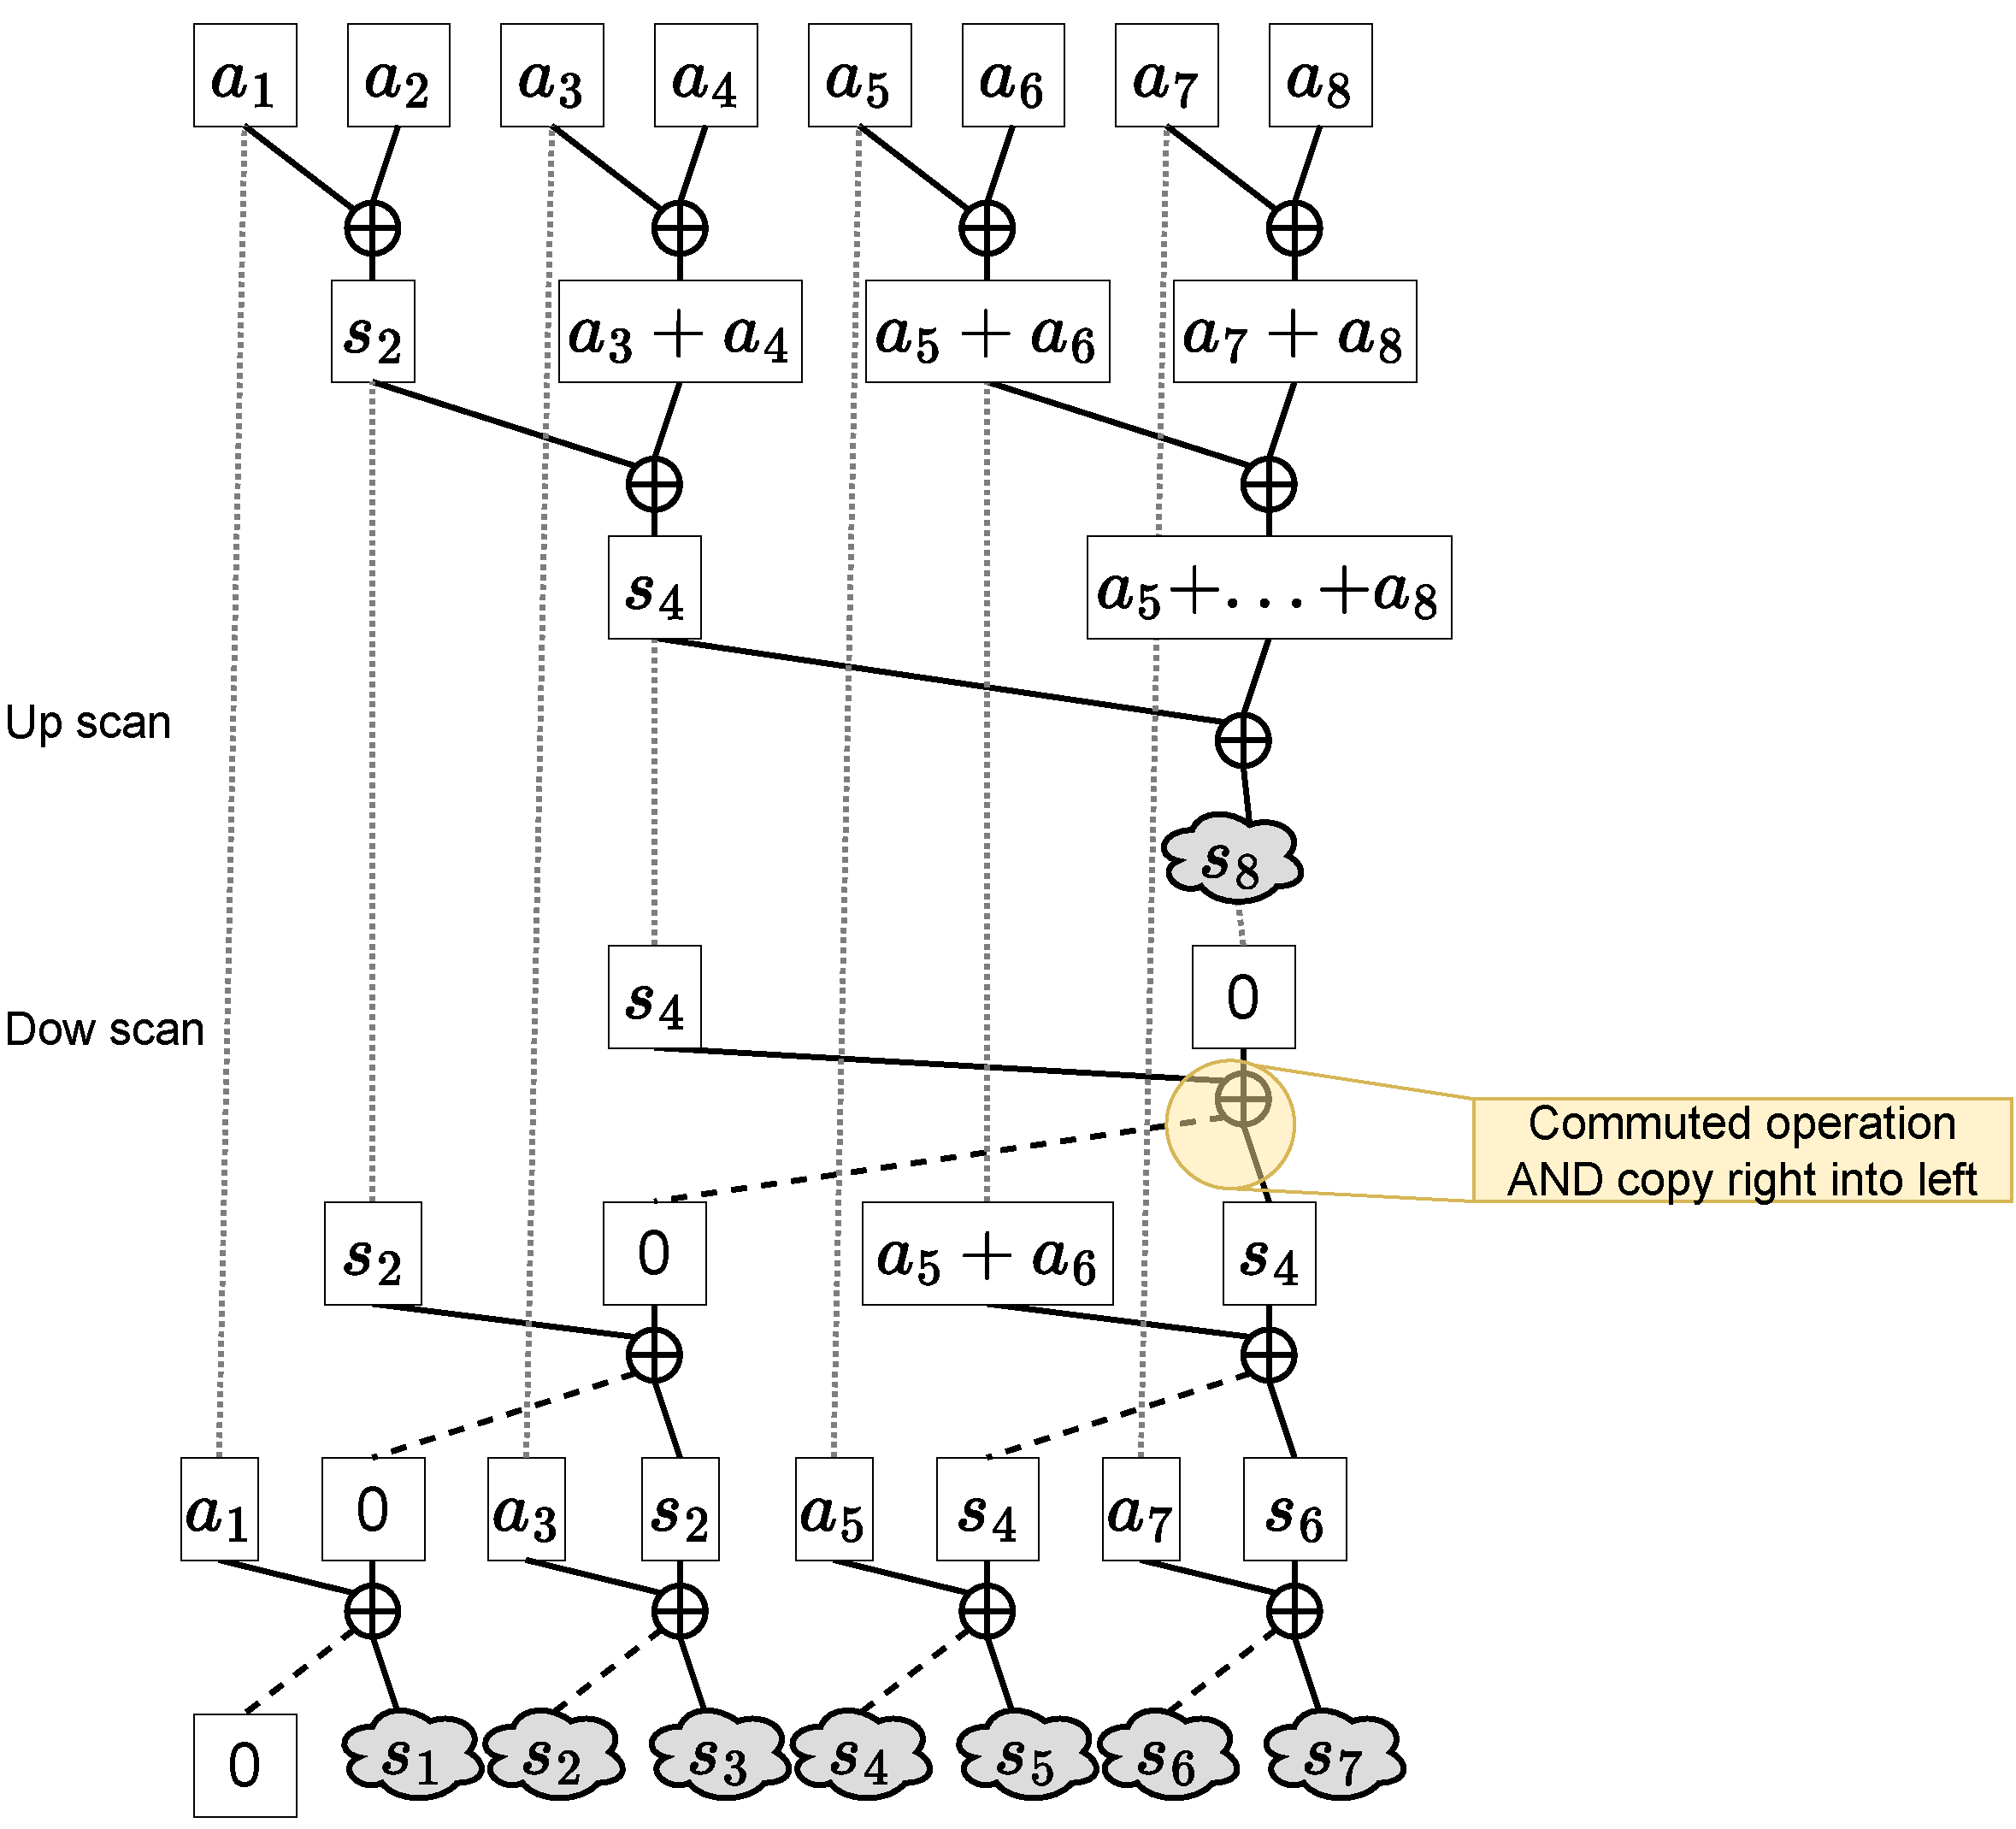
\includegraphics[height=0.3\\textheight]{figures/scan_monoid.pdf}
    \\hspace{20mm}
    \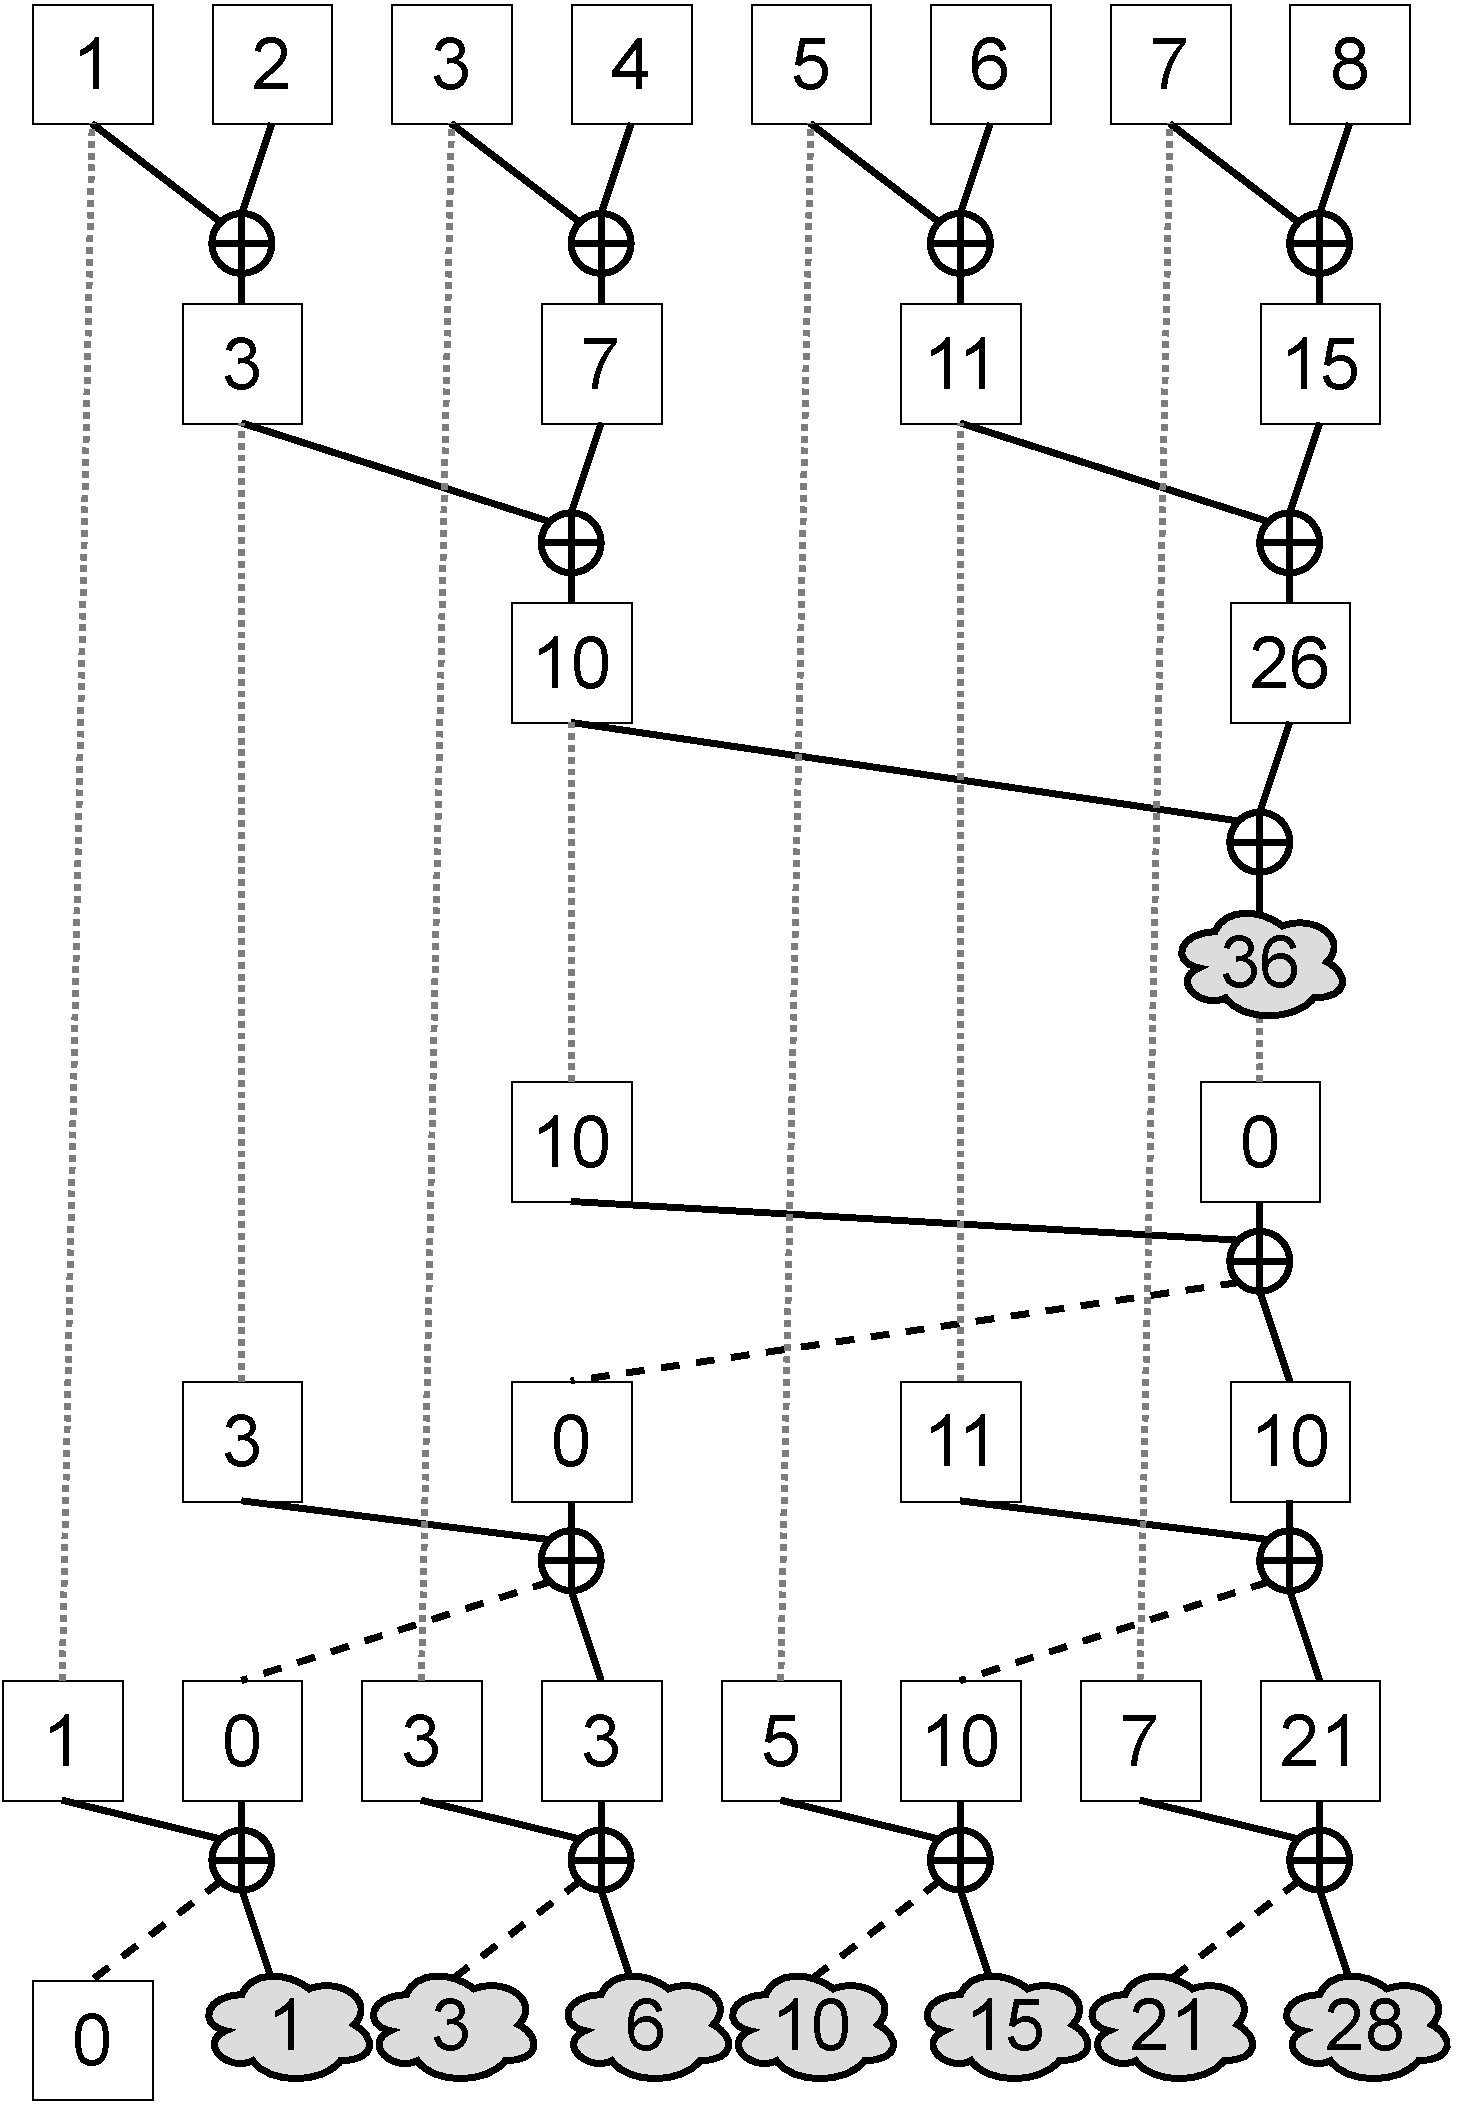
\includegraphics[height=0.3\\textheight]{figures/scan_integer.pdf}
    \\caption{\\textbf{Left:} parallel scan with a generic monoid. \\textbf{Right:} illustration on the spetial case of natural integers.}
    \\label{fig:parallel_scan_general}
\\end{figure}

\\begin{thomasbox}
PARALLEL SCAN ALGORITHM (GENERAL FORM). The parallel scan computes the cumulative sequence $(\\bigoplus_{j=0}^{i} a_j)_{i \\in I}$ in a tree structure with $O(\\log T)$ depth.

UPWARD SWEEP (UP-SWEEP): Builds a tree bottom-up. At each level $l$, pairs of adjacent elements at level $l-1$ are combined: $a^{l}_{k} = a^{l-1}_{2k} \\oplus a^{l-1}_{2k+1}$. After $\\log_2 T$ levels, the root contains $a^{\\log_2 T}_0 = \\bigoplus_{j=0}^{T-1} a_j$ (the full scan).

DOWNWARD SWEEP (DOWN-SWEEP): Distributes partial results down the tree. Starting with $b^0_1 = e$ (identity), propagate down: $(b^{l+1}_{2k}, b^{l+1}_{2k+1}) = (b^l_k, b^l_k \\oplus a^{\\log_2(T)-(l+1)}_{2k})$. At the leaves, $b^{\\log_2 T}_i$ gives the cumulative sum up to position $i$.

WHY ASSOCIATIVITY MATTERS: The tree can be reparenthesized arbitrarily as long as $\\oplus$ is associative. Non-commutativity is fine: the left-to-right order is preserved (crucial for non-commutative ops like matrix mult).

WORK: Each of the $\\log_2 T$ levels performs $T$ operations (summed over all nodes), so $W = O(T \\log T)$ in general. But when $\\oplus$ is constant-time, the work is $O(T)$.

TIME: $\\log_2 T$ levels, each parallelizable, so $T_\\infty = O(\\log T)$ assuming \\oplus is parallelizable.
\\end{thomasbox}

The procedure described above yields $(\\sum_{j=0}^{i-1}a_j)_{i\\in I}$, with the cumulative sum being $a^{\\log_2(T)}_{0}$ the intermediate result of the upward sweep. We analyse the work complexity $W$ and the time complexity $T_\\infty$ of $\\mathrm{Scan}$ in terms of floating point operations, where $W$ counts the total number of operations needed and $T_\\infty$ counts the time complexity under unlimited parallelism.

\\begin{proposition}[Parallel Scan Complexity for Integers]
\\label{prop:scan_integer_complexity}
    Let $(M, \\oplus, e) \\coloneqq (\\N, +, 0)$ be the monoid of natural integers equipped with addition. Let $(a_i)_{i\\in I}\\in \\N^I$ be a sequence of integers.

\\begin{align}
    W(\\mathrm{Scan})&= 2(T-1)\\\\\n    T_\\infty(\\mathrm{Scan})&= 2\\log_2 T
\\end{align}
\\end{proposition}

\\begin{proof}
At level $l$ of the upward scan, $U_l = T/(2^{l+1})$ $\\oplus$ operations are performed, each of them having a complexity of $1$. There are $\\log_2 T$ levels in total. The same goes on for the downward scan, with $D_l = T/(2^{\\log_2(T) - l})=2^{l}$ operations at level $l$. Therefore, the work complexity of level $l$ is $U_l$ (resp. $D_l$) while its time complexity is $1$ with unlimited parallelism. It follows that

\\begin{align}
\\label{eq:W_integer}
W &= 2\\sum_{l=0}^{\\log_2(T)-1}2^l=2(T-1)\\\\\n\\label{eq:T_integer}
T_\\infty&= 2\\sum_{l=0}^{\\log_2(T)-1}1=2\\log_2T
\\end{align}
\\end{proof}

\\begin{thomasbox}
PROOF ANNOTATION: PARALLEL SCAN FOR INTEGERS. For addition, each $\\oplus = +$ is $O(1)$.

WORK: Upward sweep has $\\log_2 T$ levels. At level $l$, there are $T/2^{l+1}$ operations. Total upward: $\\sum_{l=0}^{\\log_2 T - 1} T/2^{l+1} = T \\sum_{l=1}^{\\log_2 T} 1/2^l = T(1 - 1/2^{\\log_2 T}) = T - 1$. Similarly for downward: $T - 1$. Total: $2(T-1)$.

TIME: Each level has depth 1 (all operations at a level can happen in parallel). $\\log_2 T$ levels upward + $\\log_2 T$ levels downward = $2 \\log_2 T$.

GENERALIZATION: For $\\oplus$ taking $O(1)$ time, the work is $O(T)$ and time is $O(\\log T)$.
\\end{thomasbox}

The key point of this analysis is that the $\\oplus$ operation has constant time complexity.

\\subsection{SSM Complexity}
\\label{app:SSM_complexity}

The case of SSMs is a little more complicated than that of real numbers. In SSMs, the recurrence is defined by \\Cref{eq:ssm:recurrence}. We take $B = I$ and $d = N$ for simplicity. Thus, the goal is to compute in parallel the hidden states $(h_i = \\sum_{j=0}^i\\overline{A}^{i-j}x_j)_i\\in I$, where $x_i$ are vectors of dimension $d$ and $\\overline{A}$ is a square matrix. This is almost but not quite what we need for the parallel scan. We define the following monoid:
\\begin{align}
\\label{eq:M_SSM}
    &M^{\\mathrm{SSM}}\\coloneqq \\left\\{a = (A, x)\\mid A\\!\\in\\!\\mathcal{M}_{d}(\\R),~x\\!\\in\\!\\R^d\\right\\}\\\\\n\\label{eq:+_SSM}
    &(A_a, x_a) \\oplus^{\\mathrm{SSM}} (A_b,x_b)\\coloneqq (A_b \\odot A_a, A_b \\cdot x_a + x_b)\\\\\n\\label{eq:0_SSM}
    &e^{\\mathrm{SSM}}\\coloneqq(I_d, 0)
\\end{align}

With this monoid structure, and the sequence $(a_t)_{t\\in I} \\coloneqq ((\\overline{A}_t, x_t))_{t\\in I} \\in M^I$, the result of the parallel scan is $((A^t, \\sum_{j=0}^tA^{t-j}x_j))_{t\\in I}$. The complexity of the scan is less straightforward, but the complexity of each $\\oplus^{\\mathrm{SSM}}$ operation depends only on $d$. It is a constant of $T$. Therefore, the overall time complexity of the scan is $T_\\infty= O(\\log T)$ and $W=O(T)$.

\\begin{proposition}[SSM Complexity]
    Let $(M, \\oplus) \\coloneqq (M^{\\mathrm{SSM}}, \\oplus^{\\mathrm{SSM}})$ be the monoid defined by \\Cref{eq:M_SSM,eq:+_SSM,eq:0_SSM}. Let $(a_i)_{i\\in I}\\in (M^{\\mathrm{SSM}})^I$.

\\begin{align}
    W(\\mathrm{Scan})&= 2(T-1)(d^3+d^2+d)\\\\\n    T_\\infty(\\mathrm{Scan})&= 2\\log_2 (T) (d^3+d^2+d)
\\end{align}
\\end{proposition}

\\begin{proof}
The proof of \\Cref{prop:scan_integer_complexity} applies with the only difference that now, each $\\oplus^{\\mathrm{SSM}}$ operation has complexity $d^3$ for the matrix multiplication on the left, $d^2$ for the matrix-vector multiplication and $d$ for the vector addition on the right.
\\end{proof}

\\begin{thomasbox}
SSM MONOID AND COMPLEXITY. The monoid $(M^{\\mathrm{SSM}}, \\oplus^{\\mathrm{SSM}}, e^{\\mathrm{SSM}})$ models the recurrence $h_t = \\overline{A} h_{t-1} + \\overline{B} x_t$ as follows:

ELEMENTS: $a_t = (\\overline{A}, x_t)$. The matrix part is constant (the discretized transition matrix), and the vector part is the input at time $t$.

OPERATION: $(A_a, x_a) \\oplus (A_b, x_b) = (A_b A_a, A_b x_a + x_b)$. This combines two timesteps. Intuitively: if we have state accumulated from $(a_0 \\oplus \\ldots \\oplus a_{i-1})$ (result: $(A^{i-1}, h_{i-1})$) and next input $(a_i)$ (result: $(A, x_i)$), the combined result is $(A \\cdot A^{i-1}, A x_{i-1} + x_i) = (A^i, h_i)$.

Note: The order is left-associative. $\\oplus$ is NOT commutative (matrix mult is not commutative), but it is associative.

IDENTITY: $e = (I, 0)$. Combining with identity gives $(A, x) \\oplus (I, 0) = (A I, A \\cdot 0 + x) = (A, x)$. ✓

COMPLEXITY: Each $\\oplus$ requires:
- Matrix multiplication $A_b A_a$: $O(d^3)$
- Matrix-vector multiplication $A_b x_a$: $O(d^2)$
- Vector addition: $O(d)$
- Total per $\\oplus$: $O(d^3)$

Since this is constant w.r.t. $T$, the parallel scan work is $O(T) \\times O(d^3) = O(Td^3)$, and time is $O(\\log T) \\times O(d^3) = O(\\log T \\cdot d^3)$.

SIGNIFICANCE: For dense $A \\in \\mathbb{R}^{d \\times d}$, the $d^3$ factor is unavoidable. But for diagonal or structured $A$, this constant factor can be reduced significantly (e.g., $O(d)$ for diagonal $A$).
\\end{thomasbox}

\\subsection{Spatial ConvSSM Complexity}
\\label{app:Spatial_ConvSSM_complexity}

Rewriting the SSM (\\Cref{eq:ssm:recurrence}) to the ConvSSM formulation of \\Cref{eq:conv_ssm_discrete}, we can similarly adapt the monoid structure as :
\\begin{align}
    &M^{\\mathrm{Conv}_1}\\coloneqq \\left\\{a = (K, x)\\mid \\exists k_1, k_2,\\quad K\\!\\in\\!\\R^{k_1\\times k_2\\times c\\times c},~x\\!\\in\\!\\R^{h \\times w \\times c}\\right\\}\\\\\n    &(K_a, x_a) \\oplus^{\\mathrm{Conv}_1} (K_b,x_b)\\coloneqq (K_b \\circledast K_a, K_b \\ast x_a + x_b)\\\\\n    &e^{\\mathrm{Conv}_1}\\coloneqq(I, 0)
\\end{align}
\\noindent where $\\circledast$ is the block convolution between two kernels and $\\ast$ is the convolution between a kernel and an image:

\\begin{align*}
    & \\forall \\left\\{
\\begin{aligned}
    &i\\!\\in\\!\\intint{0}{h\\!-\\!1}\\\\\n    &j\\!\\in\\!\\intint{0}{w\\!-\\!1}\\\\\n    &c_{\\mathrm{out}}\\!\\in\\!\\intint{1}{c}
\\end{aligned}
\\right., (K\\!\\ast\\!x)_{i,j,c_{\\mathrm{out}}} = \\sum_{u=0}^{k_1-1}\\sum_{v=0}^{k_2-1}\\sum_{c_{\\mathrm{in}}=1}^{c} K_{u,v,c_{\\mathrm{in}},c_{\\mathrm{out}}} x_{(i-u,j-v)\\%(h,w),c_{\\mathrm{in}}}\\\\\n    & \\forall \\left\\{
\\begin{aligned}
    &u\\!\\in\\!\\intint{0}{k_1\\!+\\!l_1\\!-\\!2}\\\\\n    &v\\!\\in\\!\\intint{0}{k_2\\!+\\!l_2\\!-\\!2}\\\\\n    &c_{\\mathrm{in}},c_{\\mathrm{out}}\\!\\in\\!\\intint{1}{c}
\\end{aligned}
\\right., (L \\circledast K)_{u,v,c_{\\mathrm{in}},c_{\\mathrm{out}}} = \\sum_{p=0}^{l_1-1}\\sum_{q=0}^{l_2-1}\\sum_{c_{k}=1}^{c} L_{p,q,c_{k},c_{\\mathrm{out}}} K_{u-p,v-q,c_{\\mathrm{in}},c_{k}}\\text{, $K$ being zero-padded}
\\end{align*}
\\noindent with $L\\!\\in\\!\\R^{l_1\\times l_2\\times c \\times c}$, $K\\!\\in\\!\\R^{k_1\\times k_2\\times c \\times c}$ and $x\\!\\in\\!\\R^{h \\times w \\times c}$.

\\begin{thomasbox}
SPATIAL CONVSSM MONOID. This monoid models the spatial ConvSSM recurrence: $h_t = K_h \\ast h_{t-1} + K_x \\ast x_t$.

ELEMENTS: $a_t = (K, x_t)$ where $K$ is a convolution kernel (size can vary!). Note: Unlike the SSM monoid, $K$ is not fixed; it changes as the scan progresses.

OPERATION: $(K_a, x_a) \\oplus (K_b, x_b) = (K_b \\circledast K_a, K_b \\ast x_a + x_b)$. Kernel composition via block convolution.

DEFINITIONS:
- Standard convolution $K \\ast x$: apply kernel $K$ to image $x$ element-wise.
- Block convolution $L \\circledast K$: composition of two kernels. If $L$ has size $l_1 \\times l_2$ and $K$ has size $k_1 \\times k_2$, the result has size $(l_1 + k_1 - 1) \\times (l_2 + k_2 - 1)$.

EXAMPLE: If $k=3$ and two kernels are composed, result size is $3 + 3 - 1 = 5$. After $\\log_2 T$ levels, kernel size is $\\sim T \\cdot k$. This is the explosion.

IDENTITY: $e = (I, 0)$ where $I$ is the identity convolution (Dirac delta). Composing with identity gives the original kernel. ✓

WHY THE EXPLOSION MATTERS: In the parallel scan tree, at level $l$ (upward), kernels have size $O(2^l k)$. At the root (level $\\log_2 T$), kernel size is $O(2^{\\log_2 T} k) = O(Tk)$. A convolution with a $Tk \\times Tk$ kernel on a $h \\times w$ image costs $O((Tk)^2 \\times h \\times w \\times c^2) = O(T^2 k^2 hwc^2)$ FLOPs. This dominates the complexity.

EVEN WORSE: Discretization ($\\overline{K}_h = e^{\\Delta K_h}$) produces a kernel of size $h \\times w$ (full spatial support), so even at the first level, kernels are too large.
\\end{thomasbox}

With this structure, the key aspect is that the spatial size of the kernel resulting from $\\circledast$ is the sum of the sizes of the input kernels. Therefore, the parallel scan algorithm operates on larger and larger kernel sizes, with sizes growing exponentially with the depth in the tree structure. The complexity of the $\\oplus^{\\mathrm{Conv}_1}$ operator is thus no more constant as it depends on the depth. The bottleneck is at the very last layer of the upward scan, where kernel size is $O(Tk)$, with $k$ the size of the original kernels $\\overline{K}_t$, resulting in a single $\\ast$ operation whose complexity is in $O(T^2)$. This bottleneck is illustrated in \\Cref{fig:parallel_scan_conv_spatial}.

\\begin{proposition}[Spatial ConvSSM Complexity]
    Let $(M, \\oplus) \\coloneqq (M^{\\mathrm{Conv}_1}, \\oplus^{\\mathrm{Conv}_1})$ be the monoid defined by \\Cref{eq:M_SSM,eq:+_SSM,eq:0_SSM}. Let $(a_i)_{i\\in I}\\in (M^{\\mathrm{Conv}_1})^I$.

\\begin{align}
    W&= O(T^2)\\\\\n    T_\\infty&= O(W)
\\end{align}
\\end{proposition}

\\begin{proof}
The proof of \\Cref{prop:scan_integer_complexity} applies with the major difference that in the upward scan, at level $l$, each $\\oplus^{\\mathrm{Conv}_1}$ operation has complexity $(k+(2^l-1)(k-1))^2 \\times c^3 = O((2^l)^2\\times k^2 \\times c^3)$ for the kernel-kernel convolution on the left, $O(h w \\times (2^l)^2 k^2 \\times c^2)$ for the kernel-image convolution and $h w c$ for the image addition on the right. The same goes on for the downward scan.

Thus, \\Cref{eq:W_integer,eq:T_integer} become :

\\begin{align}
\\label{eq:W_conv}
W &= O(2 \\sum_{l=0}^{\\log_2(T)-1} 2^{\\log_2(T)-(l+1)} \\times \\left[ (2^l)^2 k^2 \\times c^3 + h w \\times (2^l)^2 k^2 \\times c^2\\right])\\\\\n&= O(T^2 \\times k^2 \\times c^3) + O(T^2 \\times h w \\times k^2 \\times c^2)\\\\\n\\label{eq:T_conv}
T_\\infty&= O(2\\sum_{l=0}^{\\log_2(T)-1} \\left[ (2^l)^2 k^2 \\times c^3 + h w \\times (2^l)^2 k^2 \\times c^2\\right])\\\\\n&= O(W)
\\end{align}
\\end{proof}

\\begin{thomasbox}
SPATIAL CONVSSM COMPLEXITY PROOF. The key insight: at level $l$ of the upward scan, there are $2^{\\log_2(T) - (l+1)}$ merge operations, each with kernel size $O(2^l k)$.

WORK AT LEVEL $l$:
- Kernel-kernel convolution cost: $(\\text{kernel size})^2 \\times c^3 = (2^l k)^2 c^3 = O(2^{2l} k^2 c^3)$
- Kernel-image convolution cost: $hwc^2 \\times (\\text{kernel size})^2 = hwc^2 (2^l k)^2 = O(2^{2l} hwk^2 c^2)$
- Number of operations at level $l$: $2^{\\log_2 T - (l+1)} = T/2^{l+1}$
- Total at level $l$: $\\frac{T}{2^{l+1}} \\times [O(2^{2l} k^2 c^3) + O(2^{2l} hwk^2 c^2)]$

SUMMING OVER LEVELS:
$W = \\sum_{l=0}^{\\log_2 T - 1} \\frac{T}{2^{l+1}} \\times 2^{2l} k^2 (c^3 + hwc^2) = k^2 (c^3 + hwc^2) T \\sum_{l=0}^{\\log_2 T - 1} 2^{l-1}$

The sum $\\sum_{l=0}^{\\log_2 T - 1} 2^{l-1} = 2^{-1} + 2^0 + 2^1 + \\ldots + 2^{\\log_2 T - 2} = \\sim 2^{\\log_2 T - 1} \\sim T/2$.

Thus, $W = O(T^2 k^2 c^3)$ (dominant term).

TIME: Without parallelism across levels, $T_\\infty = W = O(T^2)$ (serial bottleneck at the root).

CATASTROPHE: $O(T^2)$ is worse than sequential $O(T)$ computation! Parallel scan is completely defeated.
\\end{thomasbox}

Moreover, as mentioned in the main text, the discretization step of the SSM leads to kernels with full spatial support, meaning that the initialization of the scan is $(a_t)_{t\\in I} = ((\\overline{K}_t, x_t))_{t\\in I}$ with $\\overline{K}_t$ of size $h \\!\\times\\! w$. Thus, even the first step of the scan is intractable.

\\begin{figure}[ht]
    \\centering
    \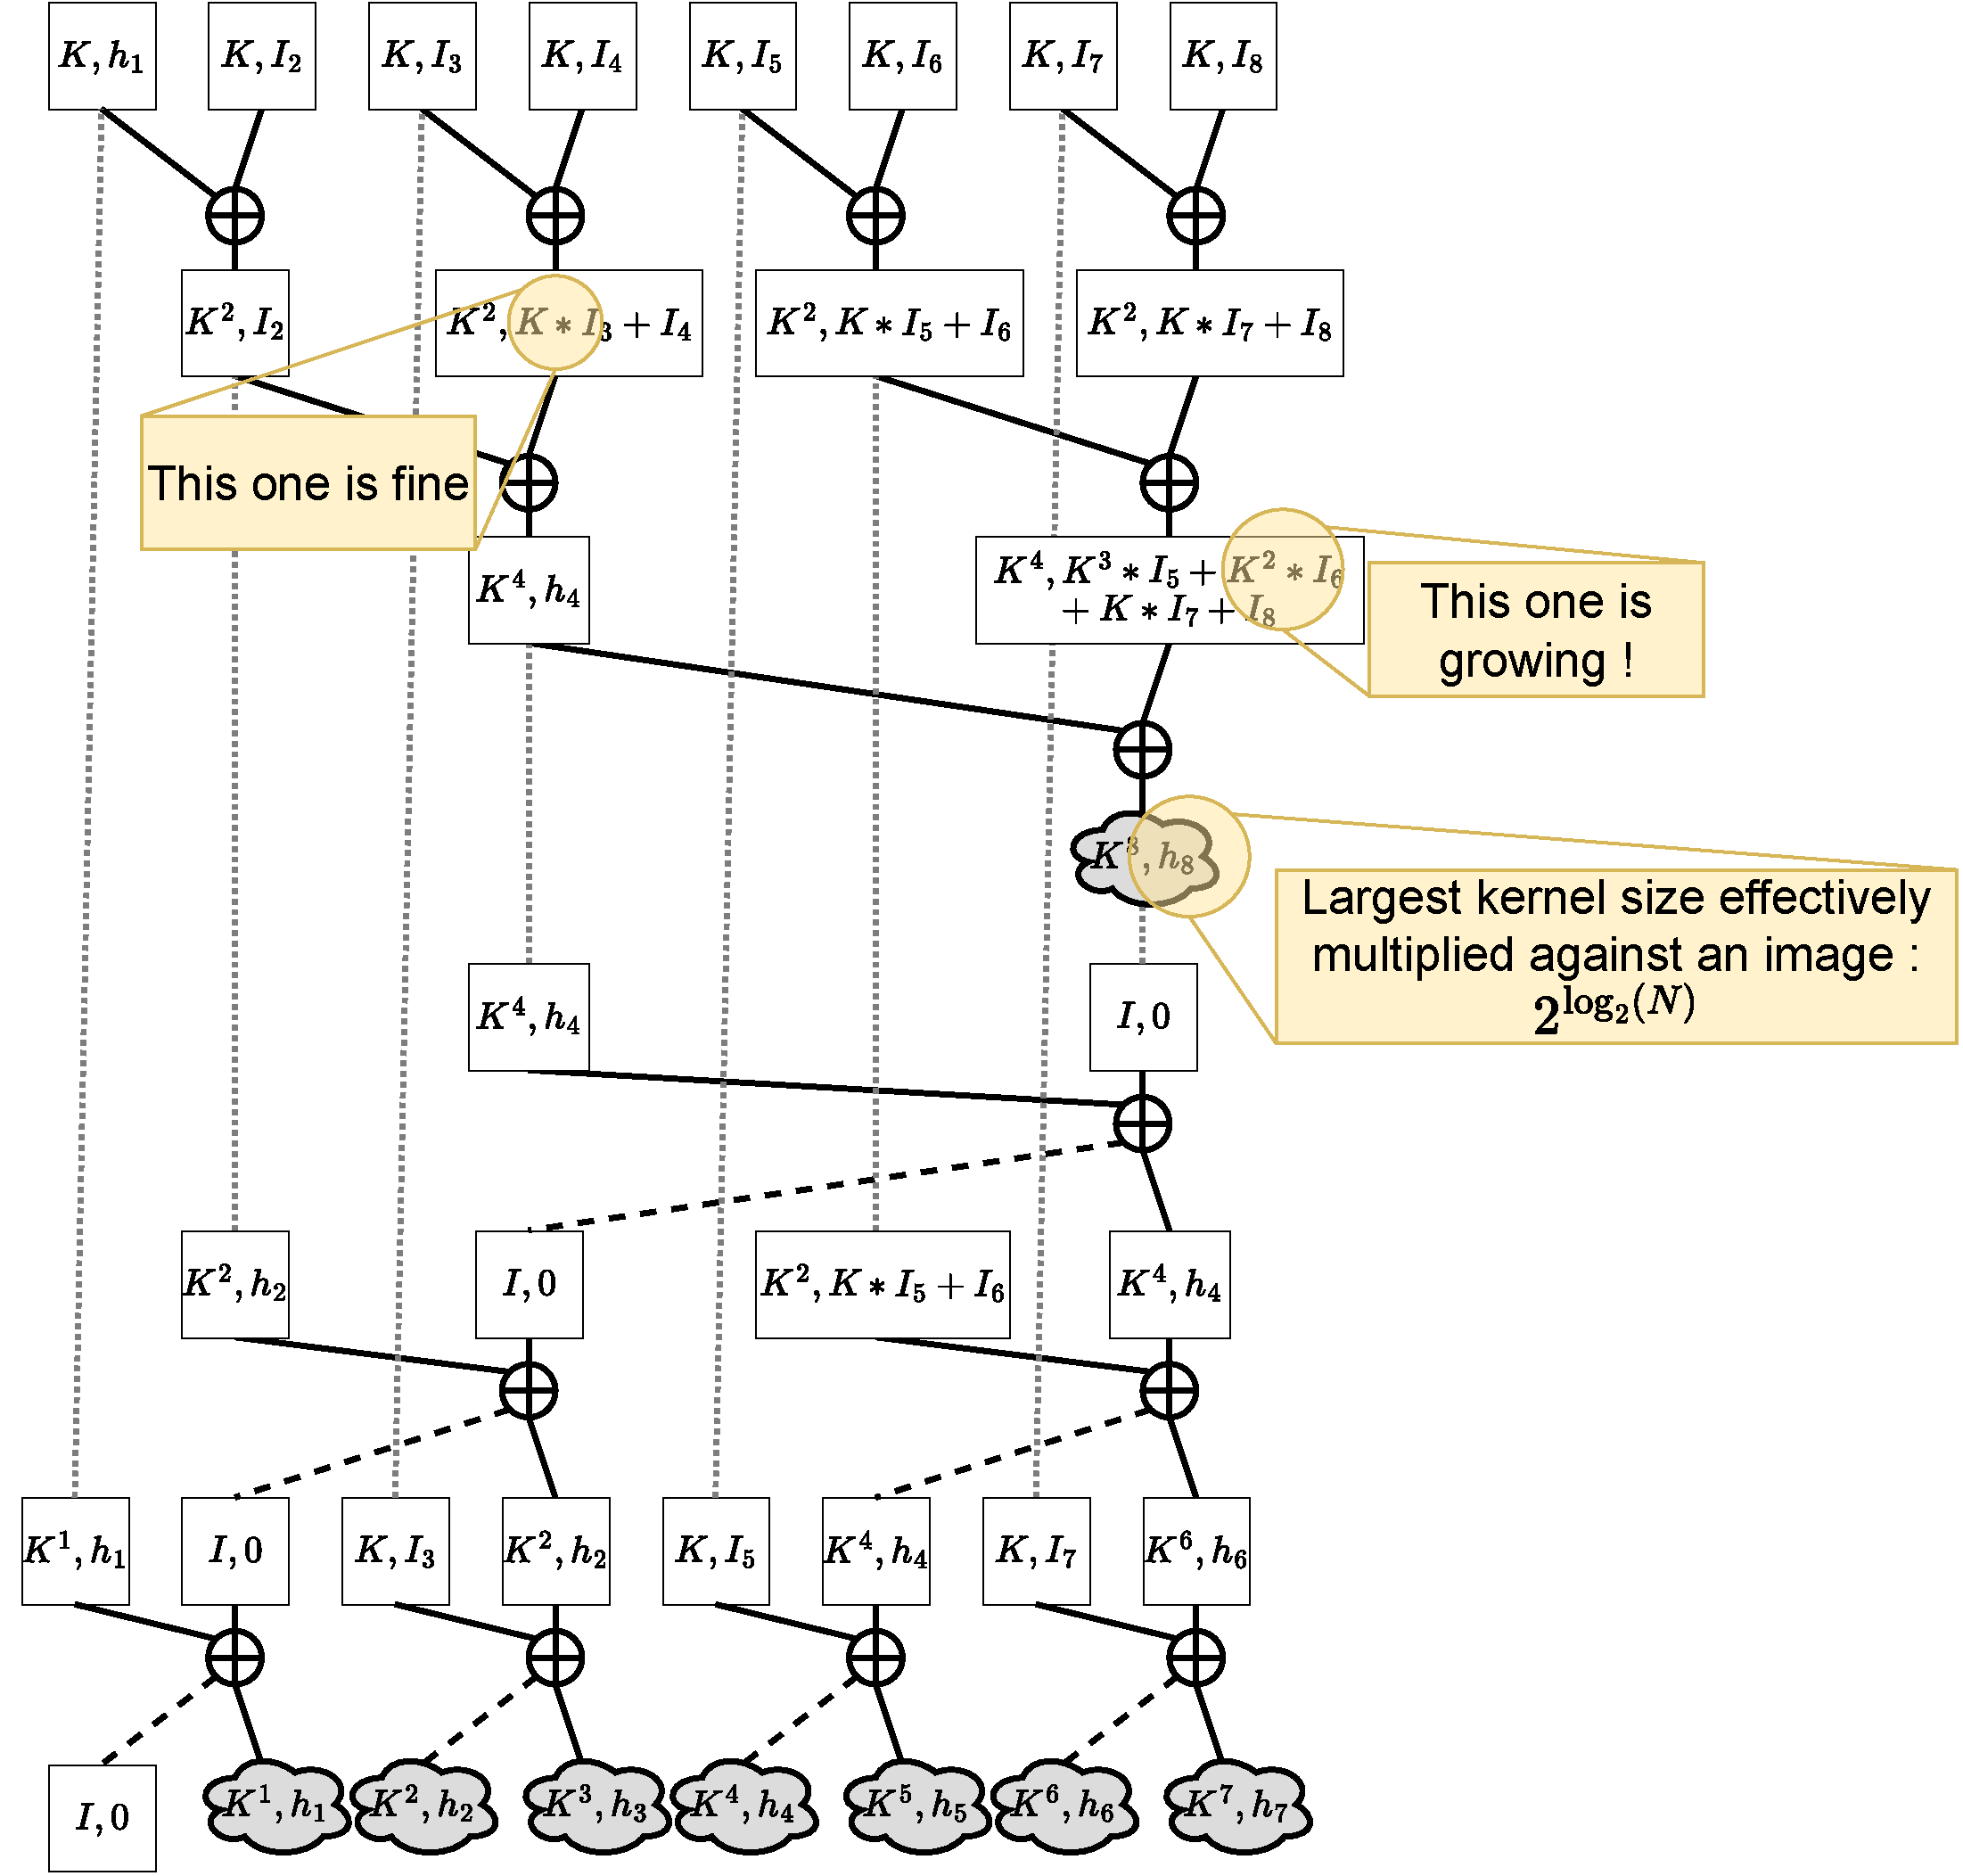
\includegraphics[height=0.3\\textheight]{figures/scan_conv.pdf}
    \\caption{Parallel scan applied to the monoid structure defined for spatial convolution SSM. Highlighted is the core of the issue : growing kernels lead to a bottleneck where a single operation has $O(T^2)$ complexity.}
    \\label{fig:parallel_scan_conv_spatial}
\\end{figure}

\\begin{thomasbox}
FULL-SPATIAL-SUPPORT DISCRETIZATION. When discretizing the spatial ConvSSM ODE using ZOH, the continuous kernel $K_h$ is replaced by $\\overline{K}_h = e^{\\Delta \\mathrm{Circ}(K_h)}$ (matrix exponential of the circulant). The result is a full-support kernel of size $h \\times w$ (the entire spatial domain).

WHY FULL SUPPORT: The matrix exponential $e^{\\Delta A}$ of a circulant matrix is also circulant. Its first row encodes the spatial kernel. For a small kernel $K_h$ (e.g., size $3 \\times 3$), the exponential $e^{\\Delta \\mathrm{Circ}(K_h)}$ has effectively non-zero entries everywhere (due to the circulant structure and the exponential function). In spectral domain, this manifests as eigenvalues with all frequencies excited.

INTRACTABILITY: A $h \\times w$ kernel cannot be applied via convolution in $O(hwk^2)$ time; it requires $O(h^2 w^2)$ time (full matrix-vector product on the stacked representation). Even the first discretization step is a bottleneck.

RESOLUTION: The spectral formulation avoids explicit kernel computation. Instead, it works directly with eigenvalues (diagonal matrix $\\Lambda$), which implicitly encode the full-support kernel but are computationally efficient.
\\end{thomasbox}

\\subsection{Spectral ConvSSM Complexity}
\\label{app:Spectral_ConvSSM_complexity}

To dispell the curse of growing kernels we move to the spectral domain and the ConvSSM formulation of \\Cref{eq:convssm}. In this domain, our monoid becomes:
\\begin{align}
\\label{eq:M_SSM_spectral}
    &M^{\\mathrm{Conv}_2}\\coloneqq \\left\\{ a = (\\Lambda_c, x)\\,\\middle|\\,\\exists (K, x')\\in M^{\\mathrm{Conv}_1},\\Bigl\\{\n\\begin{aligned}
    &\\Lambda_c = P^{-1} \\mathrm{Circ}(K_{\\mathrm{padded}}) P \\in \\C^{hwc \\times hwc}\\\\\n    &x = P^{-1} x' \\in \\C^{h w c}
\\end{aligned}
\\Bigr.\\right\\}\\\\\n\\label{eq:+_SSM_spectral}
    &(\\Lambda^a_c, x_a) \\oplus^{\\mathrm{Conv}_2} (\\Lambda^b_c, x_b)\\coloneqq (\\Lambda^b_c \\odot \\Lambda^a_c, \\Lambda^b_c \\cdot x_a + x_b)\\\\\n\\label{eq:0_SSM_spectral}
    &e\\coloneqq(I, 0)
\\end{align}
\\noindent with $\\odot$ the element-wise matrix multiplication and $\\cdot$ the element-wise matrix-vector multiplication. With this operator, the kernel grows no more, the cost is again a constant of time and depth, depending only on $h$, $w$ and $c$. We are thus back to a time complexity for the parallel scan of $O(\\log T)$.

\\begin{proposition}[Spectral ConvSSM Complexity]
    Let $(M, +) \\coloneqq (M^{\\mathrm{Conv}_2}, \\oplus^{\\mathrm{Conv}_2})$ be the monoid defined by \\Cref{eq:M_SSM_spectral,eq:+_SSM_spectral,eq:0_SSM_spectral}. Let $(a_i)_{i\\in I}\\in (M^{\\mathrm{Conv}_2})^I$.

\\begin{align}
    W&= O(T)\\\\\n    T_\\infty&= O(\\log_2T)
\\end{align}
\\end{proposition}

\\begin{proof}
The proof of \\Cref{prop:scan_integer_complexity} applies with the only difference that now, each $\\oplus^{\\mathrm{Conv}_2}$ operation has complexity $h w c^3$ for the kernel-kernel multiplication on the left, $h w c^2$ for the kernel-image multiplication and $h w c$ for the image addition on the right. This gives :

\\begin{align}
\\label{eq:W_spectral}
    W&= O(T \\times h w c^3)\\\\\n\\label{eq:T_spectral}
    T_\\infty&= O(\\log_2T \\times h w c^3)
\\end{align}
\\end{proof}

\\begin{thomasbox}
SPECTRAL CONVSSM MONOID AND COMPLEXITY. The key idea: instead of composing spatial kernels $K_a \\circledast K_b$ (which grow), compose spectral block-diagonal matrices $\\Lambda^a_c \\odot \\Lambda^b_c$ (fixed size).

ELEMENTS: $a_t = (\\Lambda^t_c, x_t)$ where $\\Lambda^t_c$ is the block-diagonal Fourier representation of the kernel at time $t$.

OPERATION: $(\\Lambda^a_c, x_a) \\oplus (\\Lambda^b_c, x_b) = (\\Lambda^b_c \\odot \\Lambda^a_c, \\Lambda^b_c \\cdot x_a + x_b)$.

KEY PROPERTIES:
- $\\odot$ is element-wise multiplication of matrices (or Hadamard product per block). Two block-diagonal matrices compose to a block-diagonal matrix of the same size.
- $\\Lambda^b_c \\odot \\Lambda^a_c$ has size $hwc \\times hwc$ (unchanged by composition).
- Cost: $hwc^3$ for the block mult, $hwc^2$ for block-matrix-vector mult.

WORK: $O(T)$ level-wise operations, each $O(hwc^3)$, total $O(T hwc^3)$.

DEPTH: $\\log_2 T$ levels, each with depth $O(hwc^3)$, but since this is per-operation (not parallelizable within the operation), actual depth is $O(\\log_2 T \\times hwc^3)$ if operations are sequential. But typically, the block operations are parallelizable (e.g., element-wise ops), so depth is closer to $O(\\log_2 T)$.

COMPARISON TO SPATIAL:
- Spatial: $W = O(T^2 k^2 c^3)$, $T_\\infty = O(T^2)$. Terrible.
- Spectral: $W = O(T hwc^3)$, $T_\\infty = O(\\log_2 T \\times hwc^3) \\approx O(\\log_2 T)$ for large $T$. Excellent.

The spectral approach recovers the logarithmic-depth parallel scan while maintaining spatial coupling (horizontal connections). This is the main contribution.
\\end{thomasbox}

\\subsection{Taking down the constant factors}
\\label{app:constant_factors}

Now that we have solved the main issue of complexity explosion with time, we tackle the problem of the constant factor. As mentioned in \\Cref{prop:SSM_complexity}, as is, the work complexity is $O(T)$ with a constant that is $O(d^3)$ due to matrix multiplications.
%
The diagonal SSM (\\Cref{eq:ssm:diagonal}) reduces this constant from $O(d^3)$ to $O(d)$. The complexity gain comes from the change of basis being absorbed outside of the recurrence such that the recurrence can operate on diagonalized matrices.

In the case of the Spectral SSM (\\Cref{eq:ssm:spectral}), the $O(c^3)$ is even more prohibitive as it is repeated over each pixel position, with the total constant being $O(hwc^3)$ in the spectral domain (\\Cref{eq:W_spectral,eq:T_spectral}). Hence the diagonal spectral SSM (\\Cref{eq:ssm:diagonal_spectral}), which reduces the constant to $O(hwc)$. Our ConvSSM formulation (\\Cref{eq:convssm}) exploits this diagonal spectral SSM and couples it with convolutional input and output transforms in order to make the whole model tractable.

\\begin{thomasbox}
REDUCING CONSTANT FACTORS: FROM $O(hwc^3)$ TO $O(hwc)$. The spectral ConvSSM has complexity $O(T hwc^3)$, which is still expensive. The bottleneck is the $c^3$ term from composing block-diagonal matrices.

SOLUTION: Apply a second diagonalization to the block-diagonal $\\Lambda_c = Q_c \\Lambda Q_c^{-1}$, where $\\Lambda$ is fully diagonal and $Q_c$ is block-diagonal. Then, the composition is:
$(\\Lambda_c)^b \\odot (\\Lambda_c)^a = (Q_c \\Lambda^b Q_c^{-1}) \\odot (Q_c \\Lambda^a Q_c^{-1})$

Rearranging: $Q_c (\\Lambda^b \\odot \\Lambda^a) Q_c^{-1} = Q_c \\Lambda^{b+a} Q_c^{-1}$ (since $\\Lambda^b \\odot \\Lambda^a = \\Lambda^{b+a}$ element-wise for diagonal matrices).

But wait: with full diagonalization, the $\\oplus$ operation becomes:
$(\\Lambda^a, x_a) \\oplus (\\Lambda^b, x_b) = (\\Lambda^b \\odot \\Lambda^a, \\ldots)$

The composition is now element-wise multiplication (diagonal by diagonal), costing $O(N) = O(hwc)$ for a single vector.

COST TRANSFER: The diagonalization cost is moved to the input/output transforms $\\widetilde{B}$ and $\\widetilde{C}$. But these are applied once per sequence (or cached), amortizing the cost.

FINAL COMPLEXITY: Parallel scan work: $O(T hwc)$. Amortized per-step cost: $O(hwc)$. Plus FFT overhead: $O(T \\log(hw) c)$ for input/output transforms. Total: $O(T hwc + T \\log(hw) c) = O(T hwc)$ (linear in sequence length, spatial size, and channels).

COMPARISON TO DENSE SSM:
- Dense SSM: $O(T d^3) = O(T (hwc)^3)$. Impractical for high-resolution images.
- Spectral ConvSSM: $O(T hwc)$. Practical.

This is the key algorithmic contribution: reducing a cubic-in-spatial-dimension cost to linear.
\\end{thomasbox}

\\end{document}
